\appendix
\chapter{Appendices}
\section{$Z\to\tauh\mu$ final state distributions}
\begin{figure}[H]
	\centering
	\subfloat[]{\label{Fig17a}{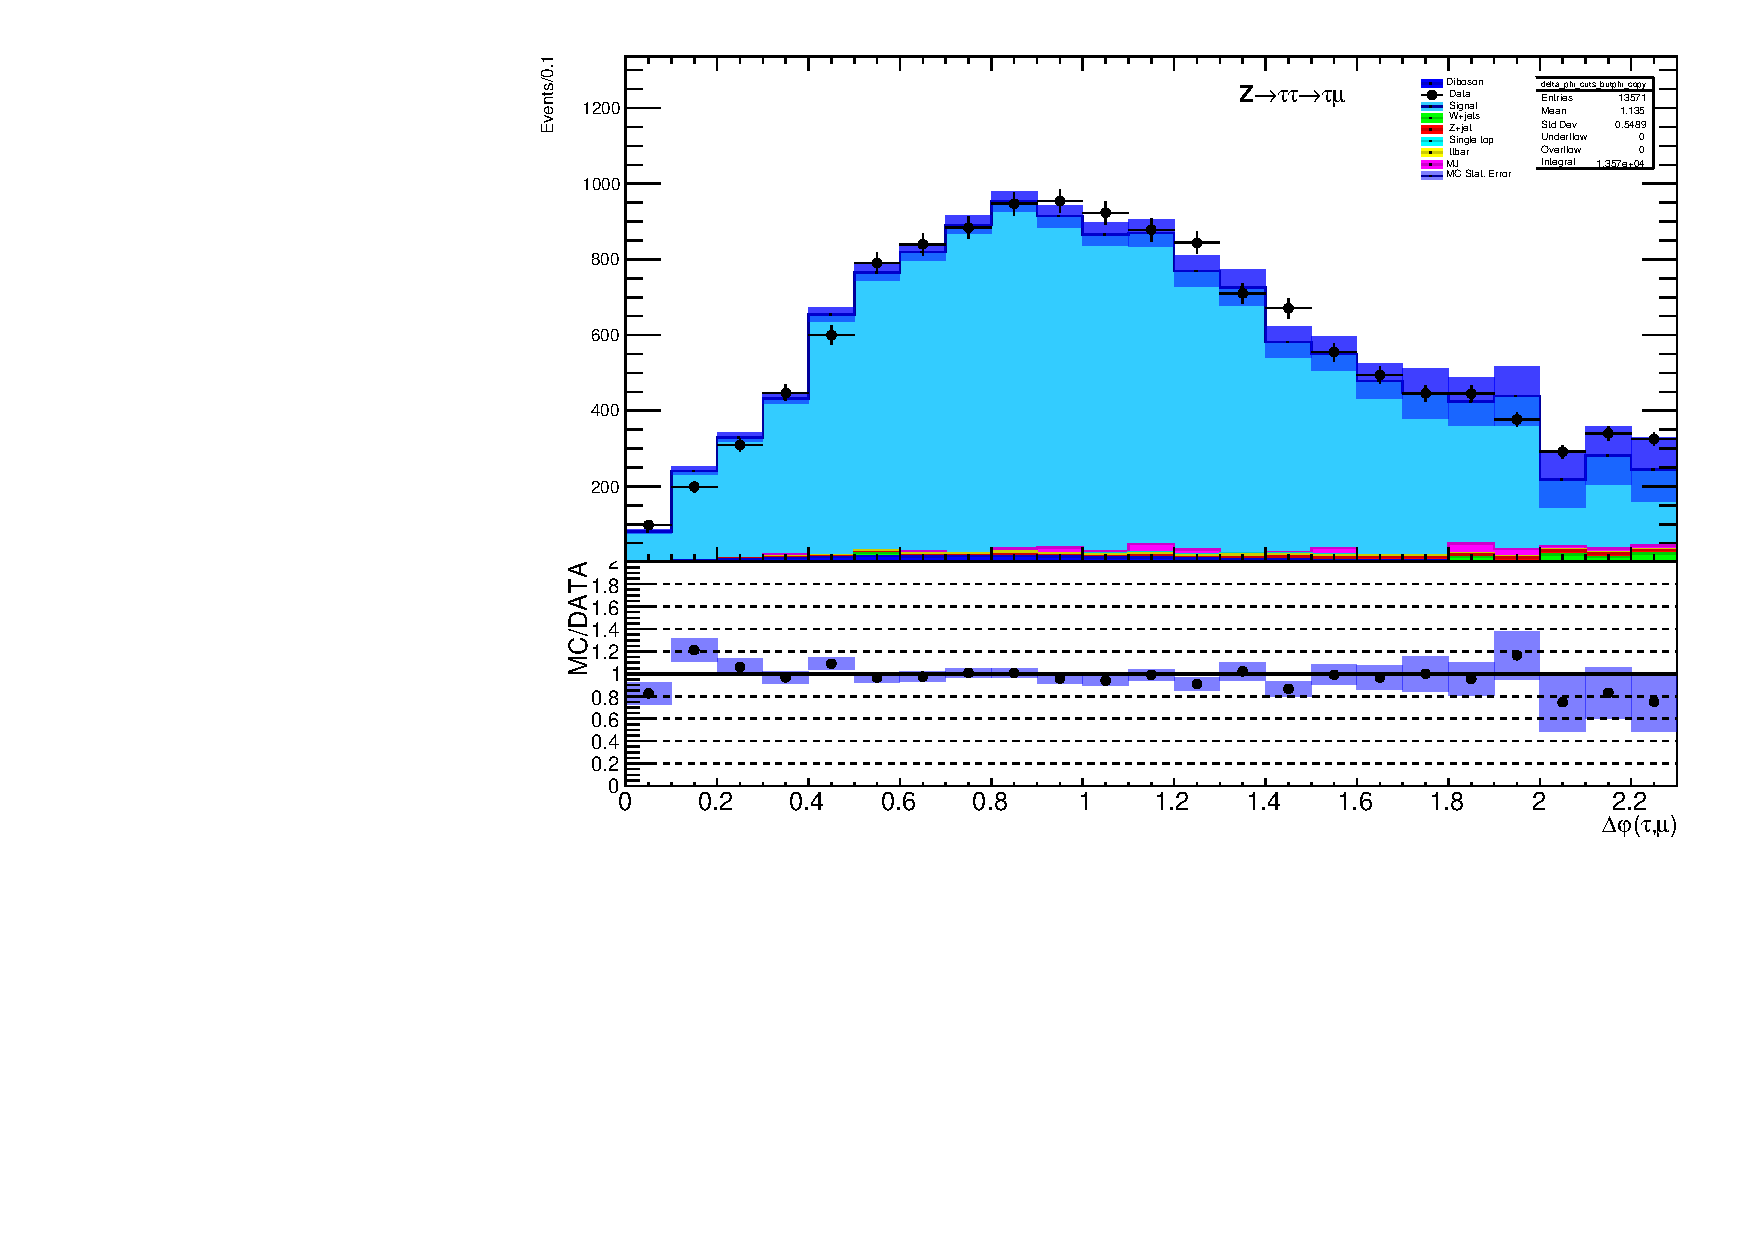
\includegraphics[width=0.50\textwidth]{figures/Fig17a}}}\hfill
	\subfloat[]{\label{Fig17b}{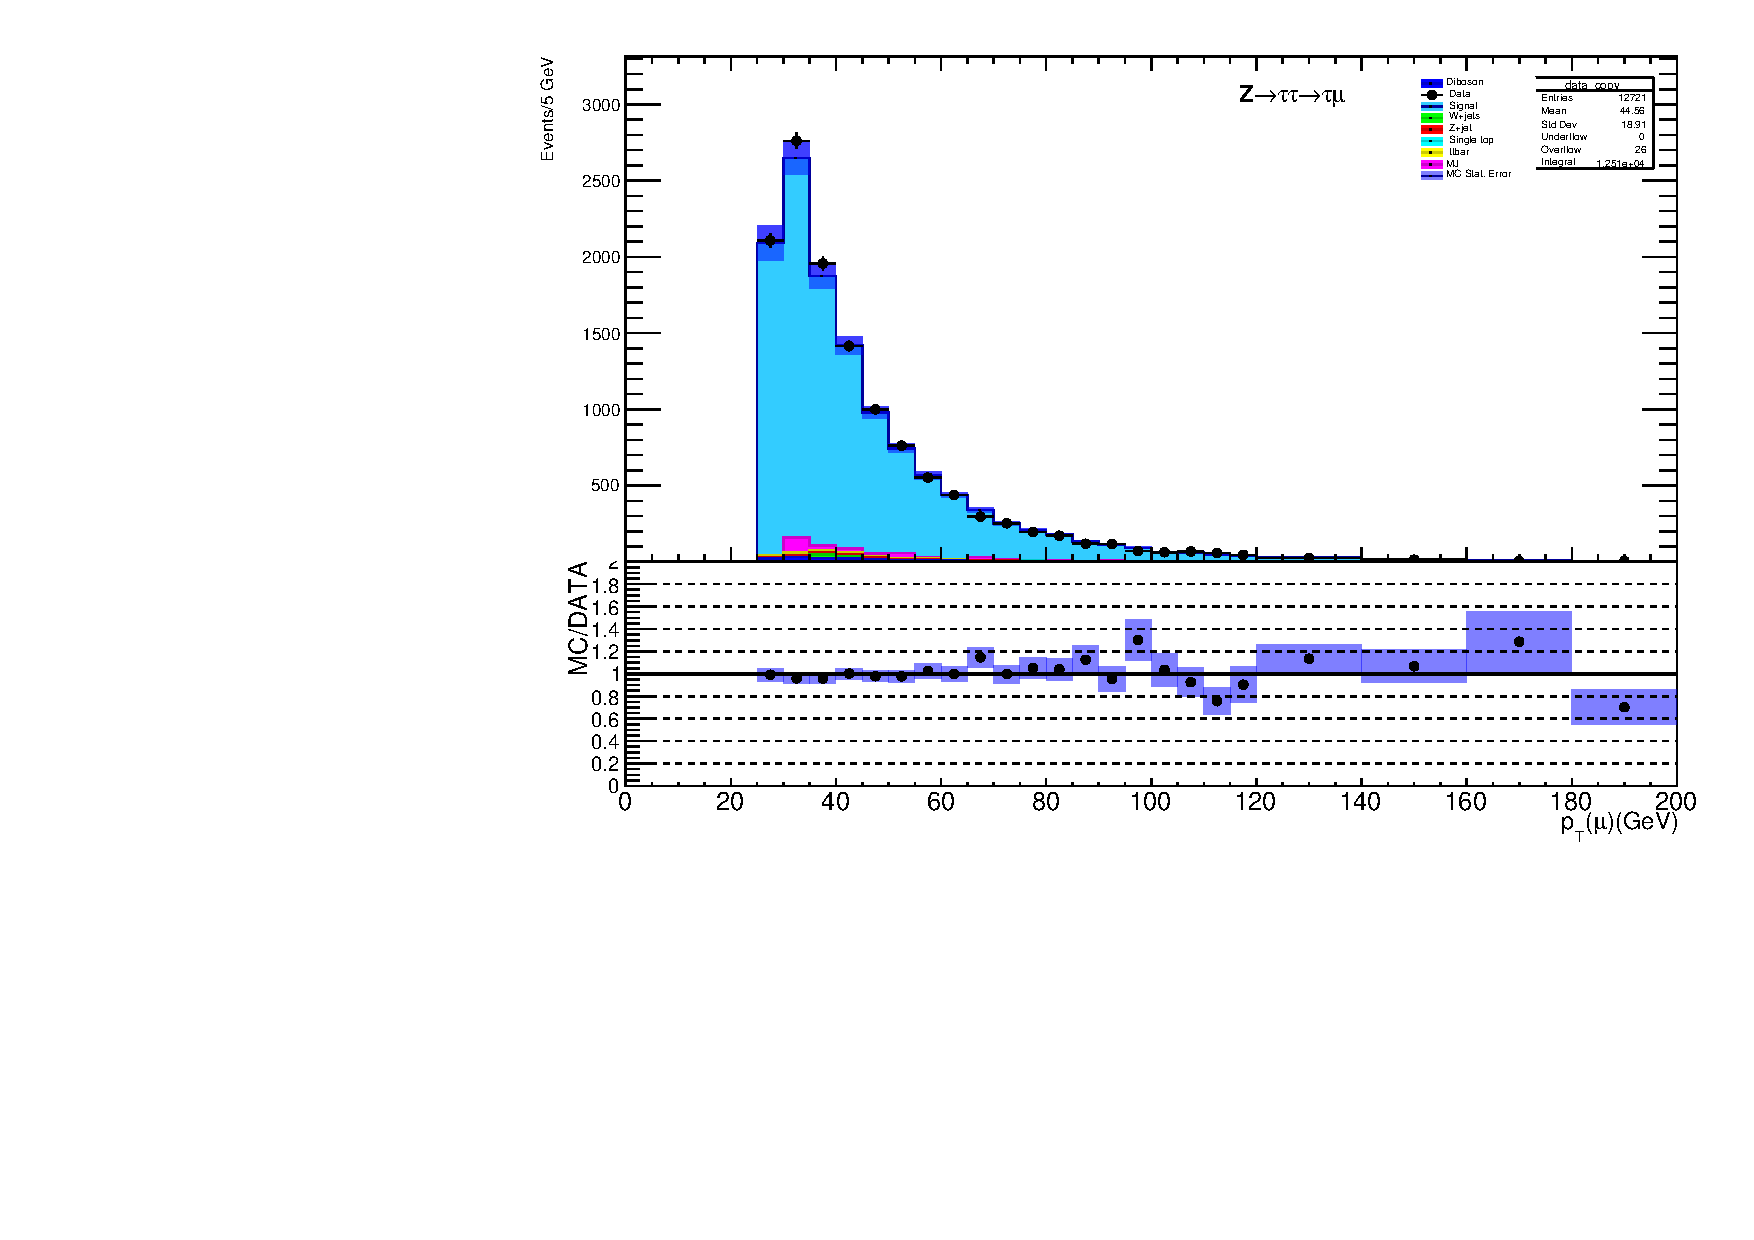
\includegraphics[width=0.50\textwidth]{figures/Fig17b}}}\hfill
	\subfloat[]{\label{Fig17c}{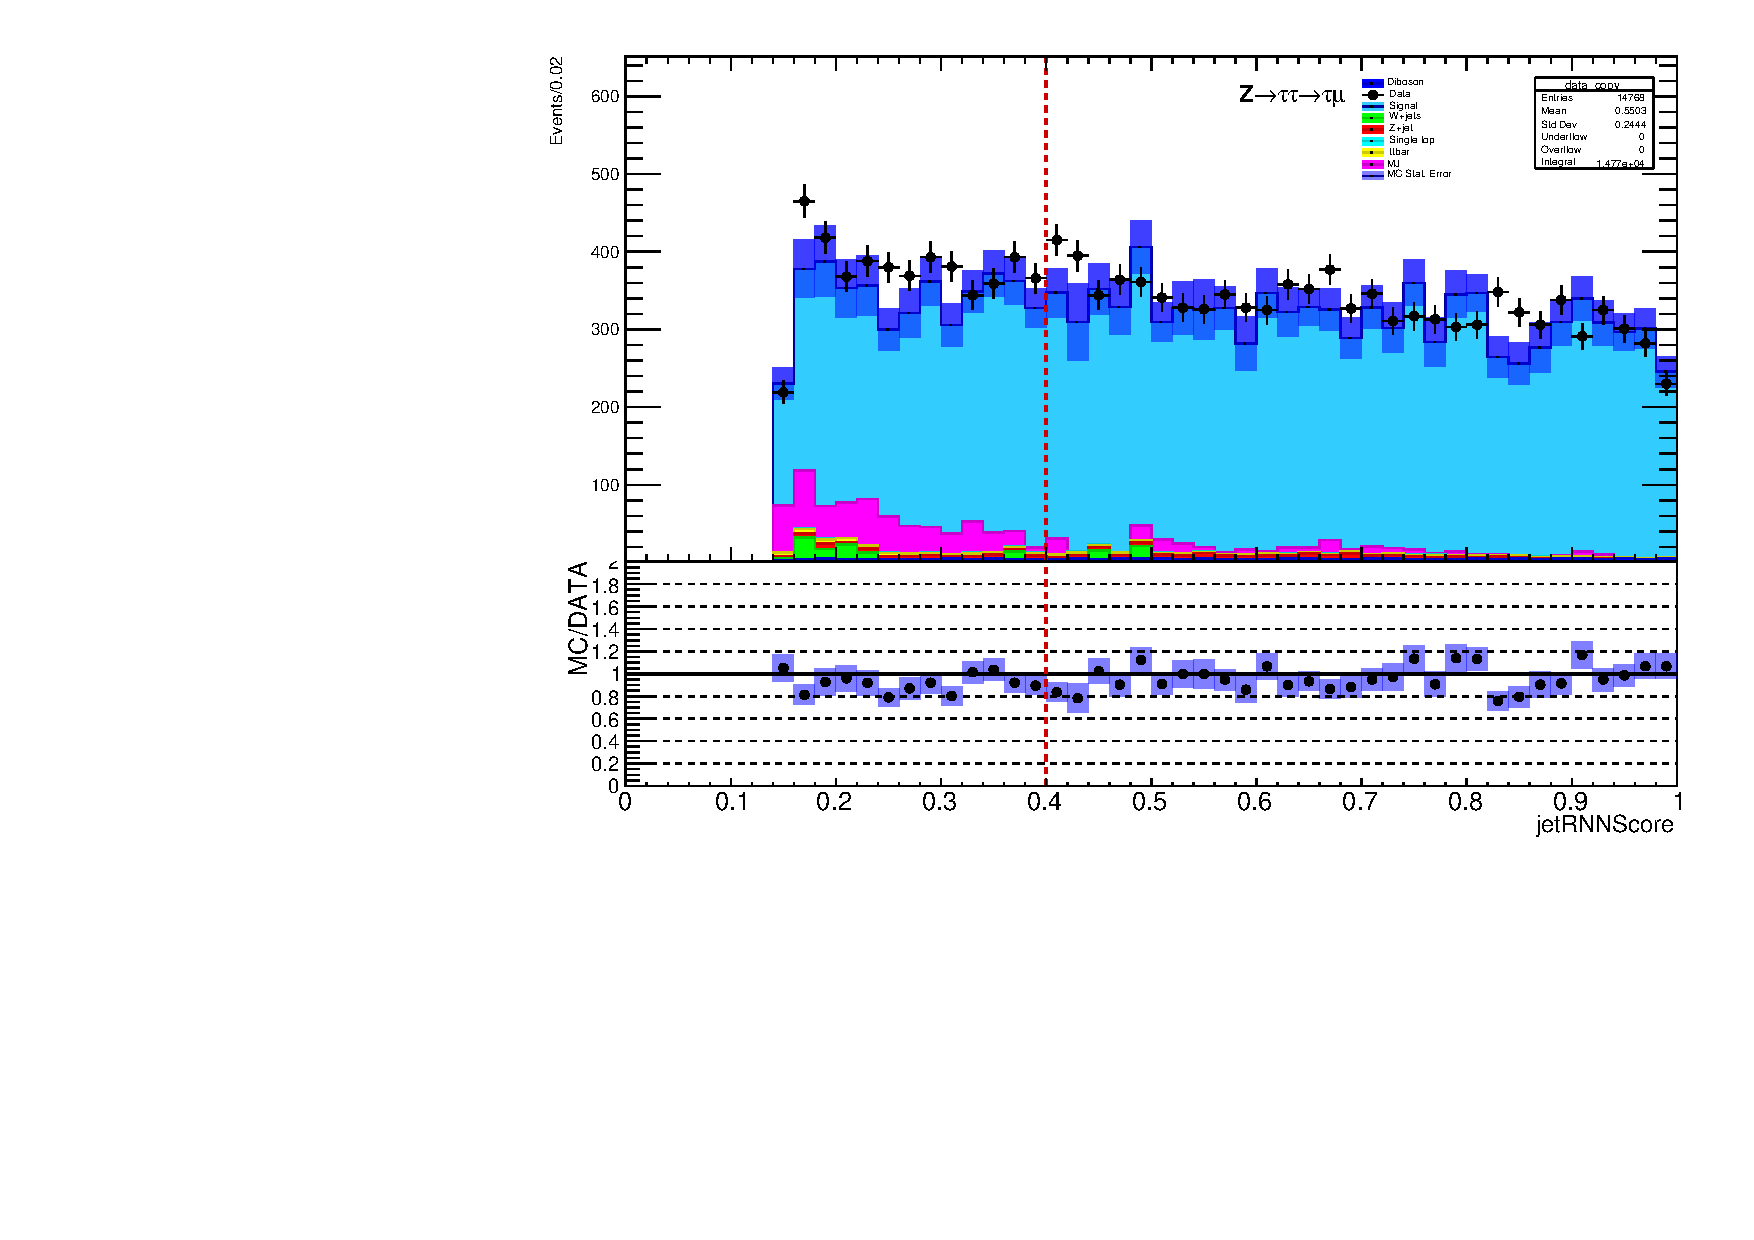
\includegraphics[width=0.50\textwidth]{figures/Fig17c}}}\hfill
	\subfloat[]{\label{Fig17d}{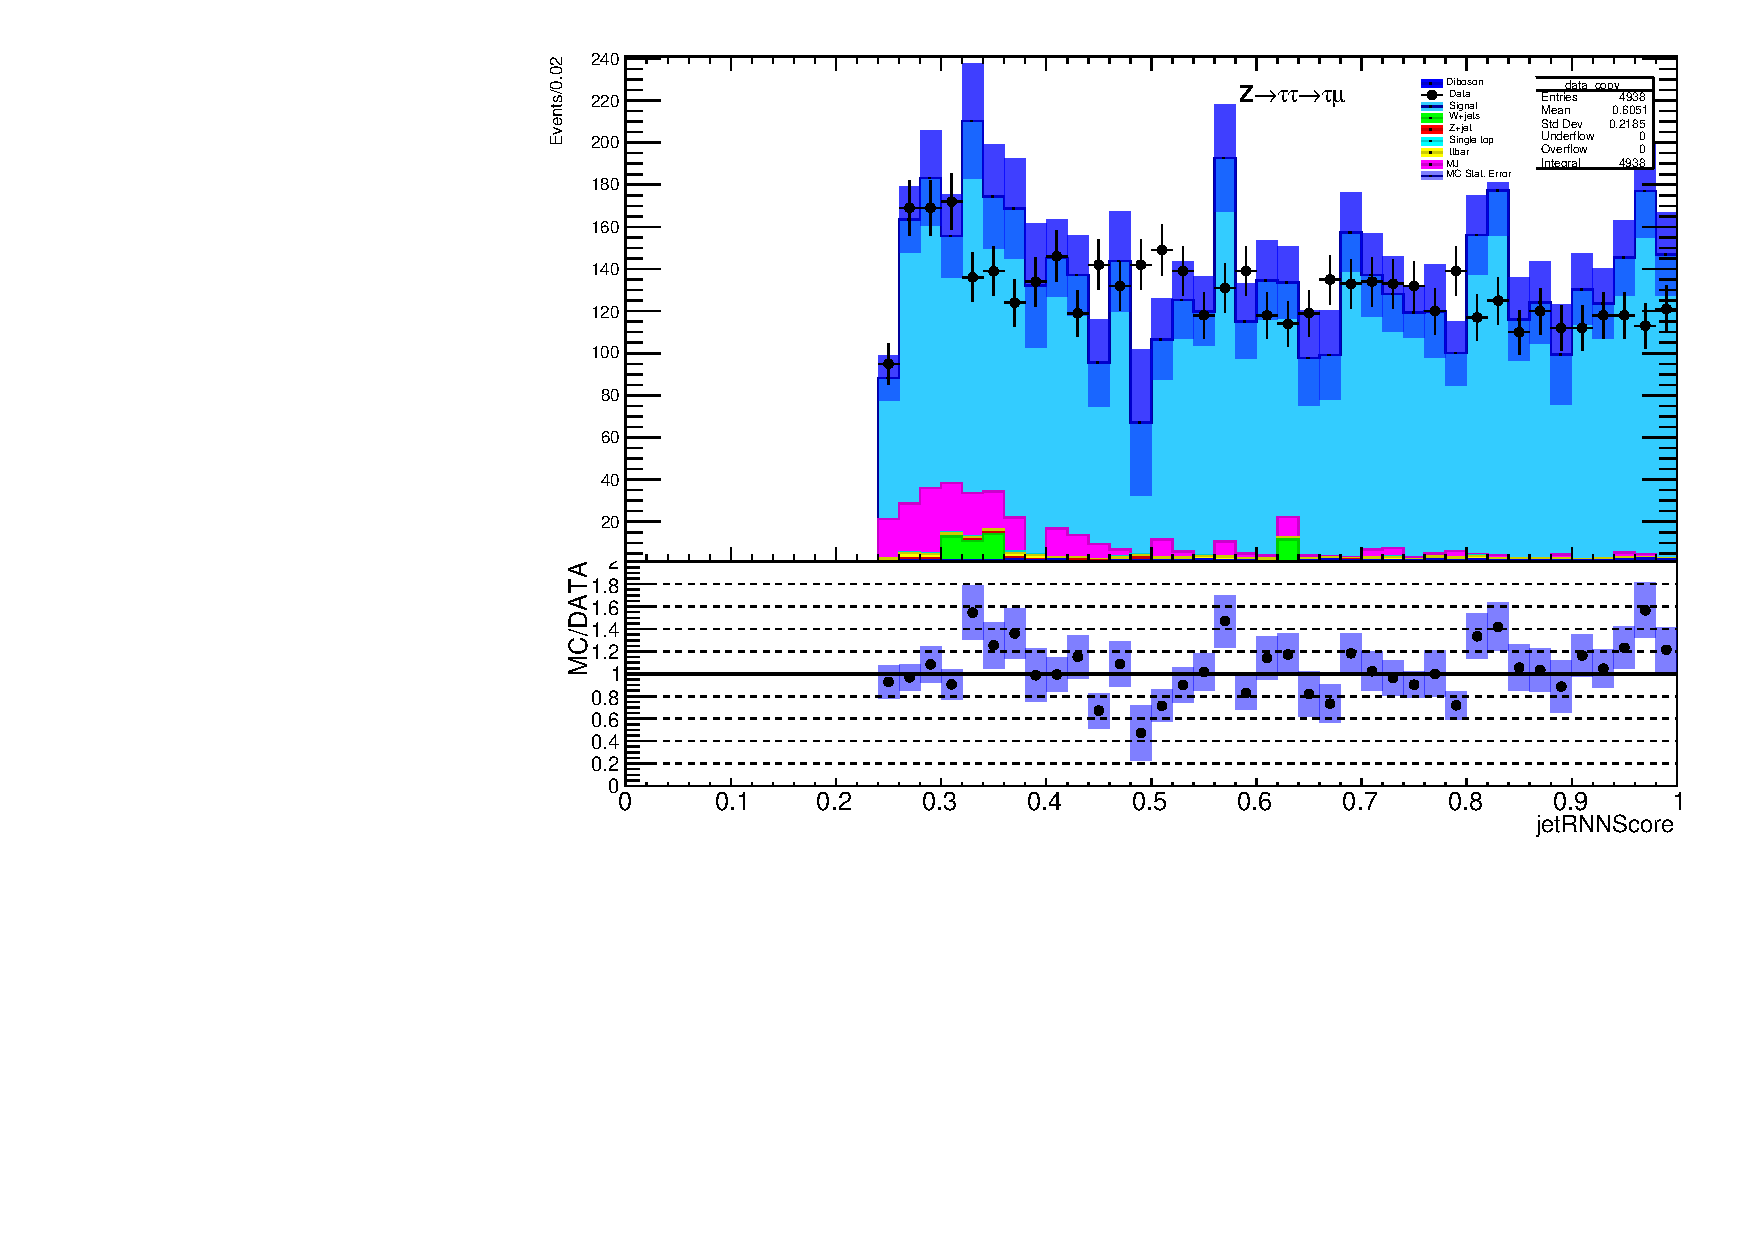
\includegraphics[width=0.50\textwidth]{figures/Fig17d}}}\hfill
	\subfloat[]{\label{Fig17e}{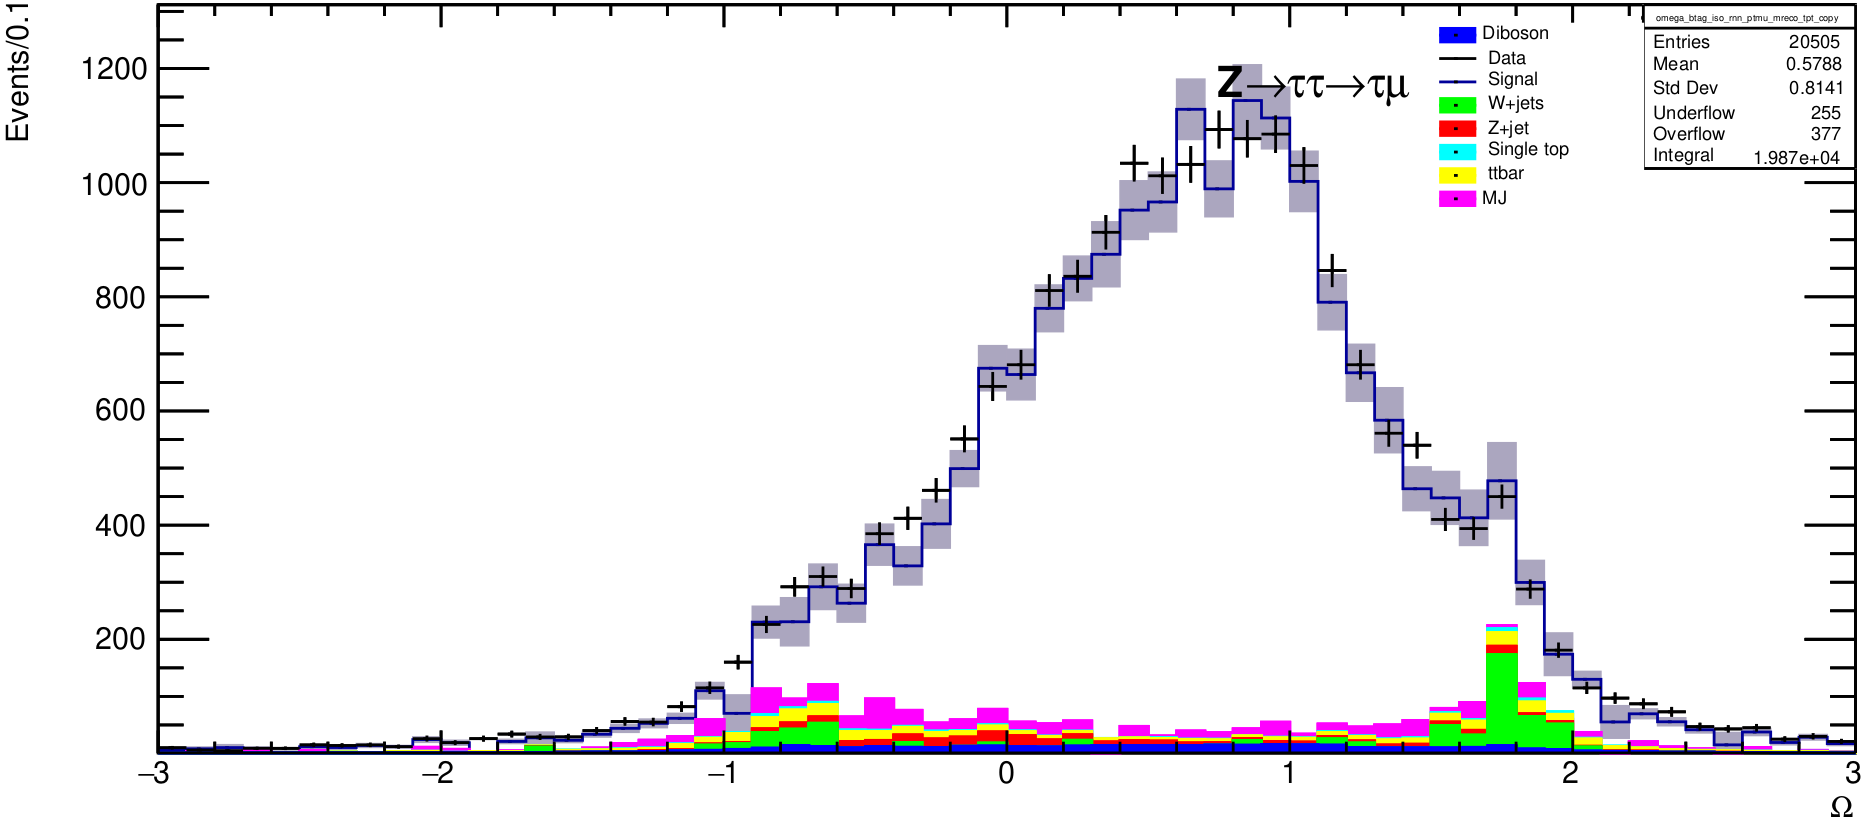
\includegraphics[width=0.50\textwidth]{figures/Fig9}}}\hfill
	\subfloat[]{\label{Fig17f}{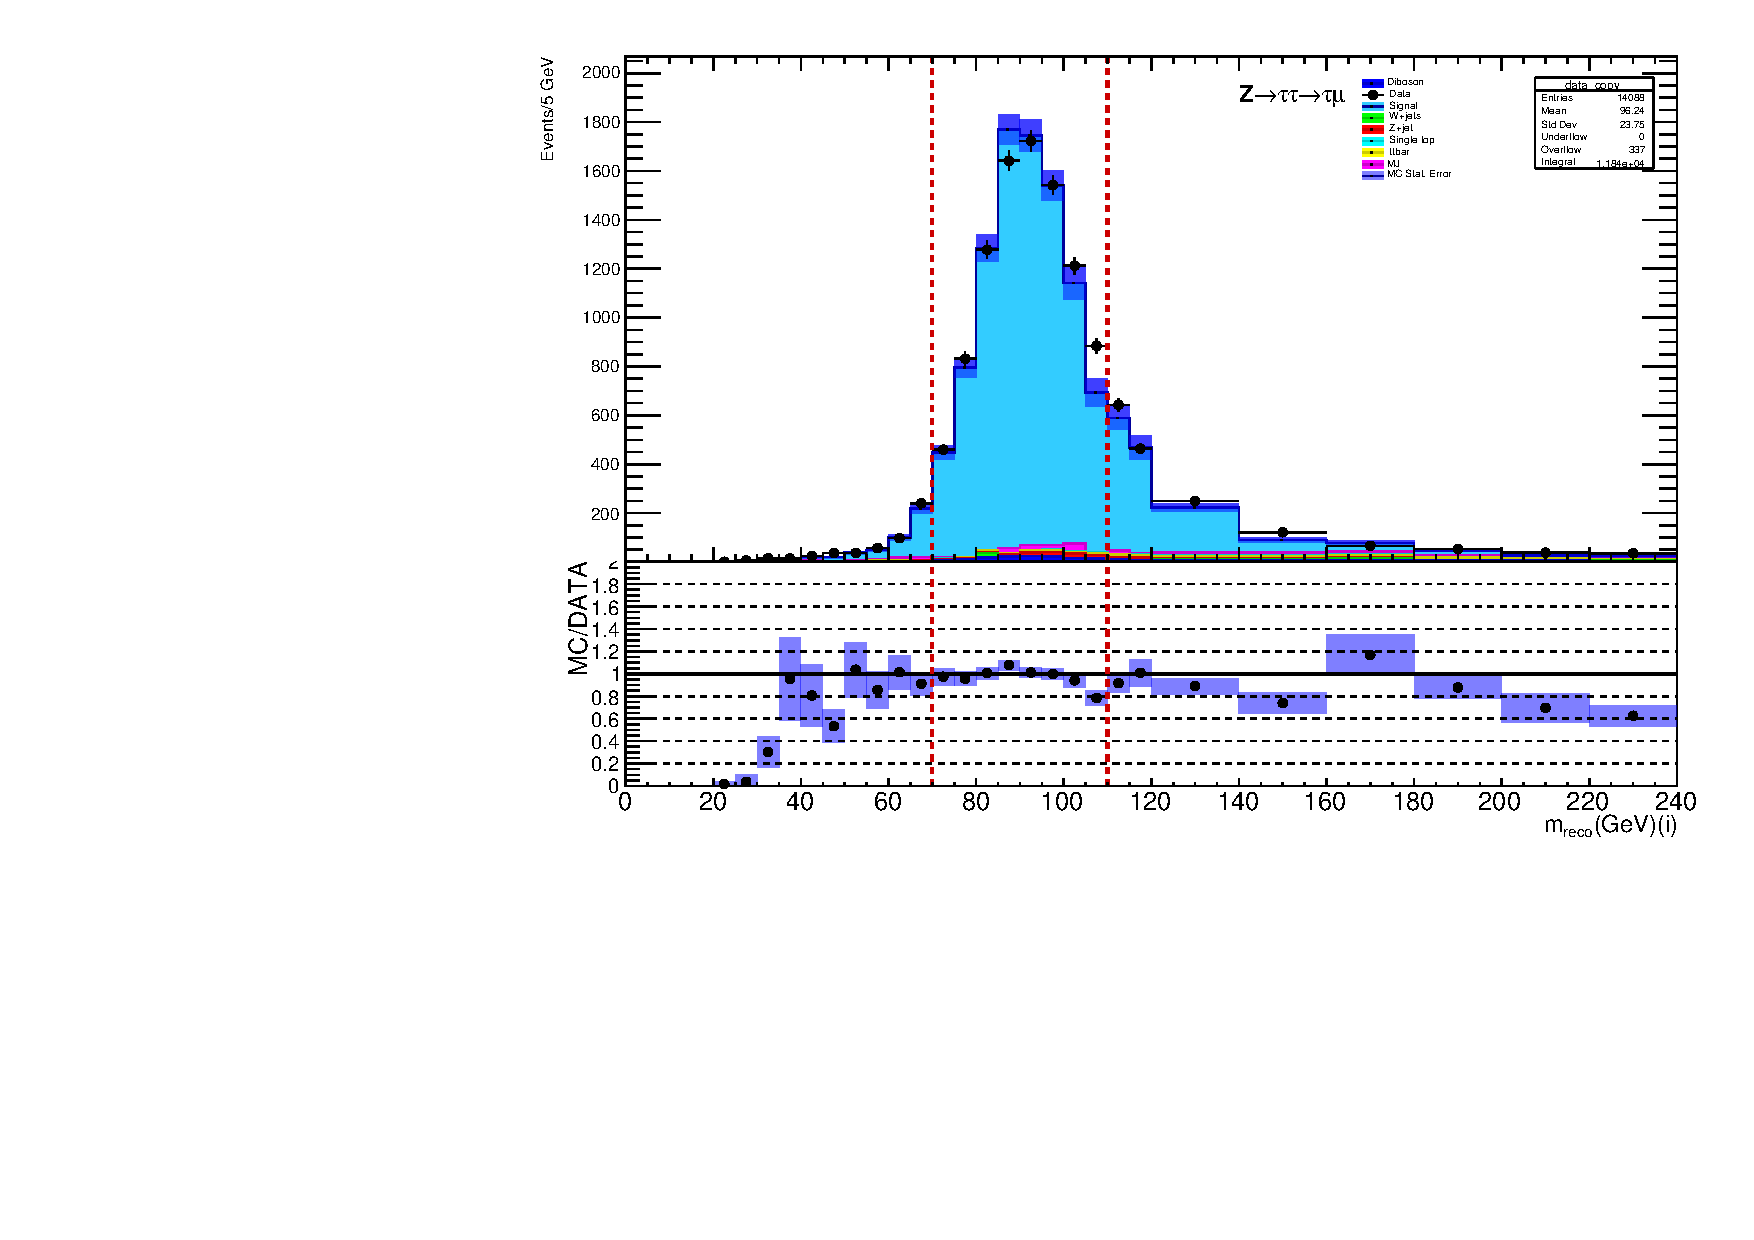
\includegraphics[width=0.50\textwidth]{figures/Fig17f}}}
	\label{Fig17}
\end{figure}
\begin{figure}[H]\ContinuedFloat
	\centering
	\subfloat[]{\label{Fig17g}{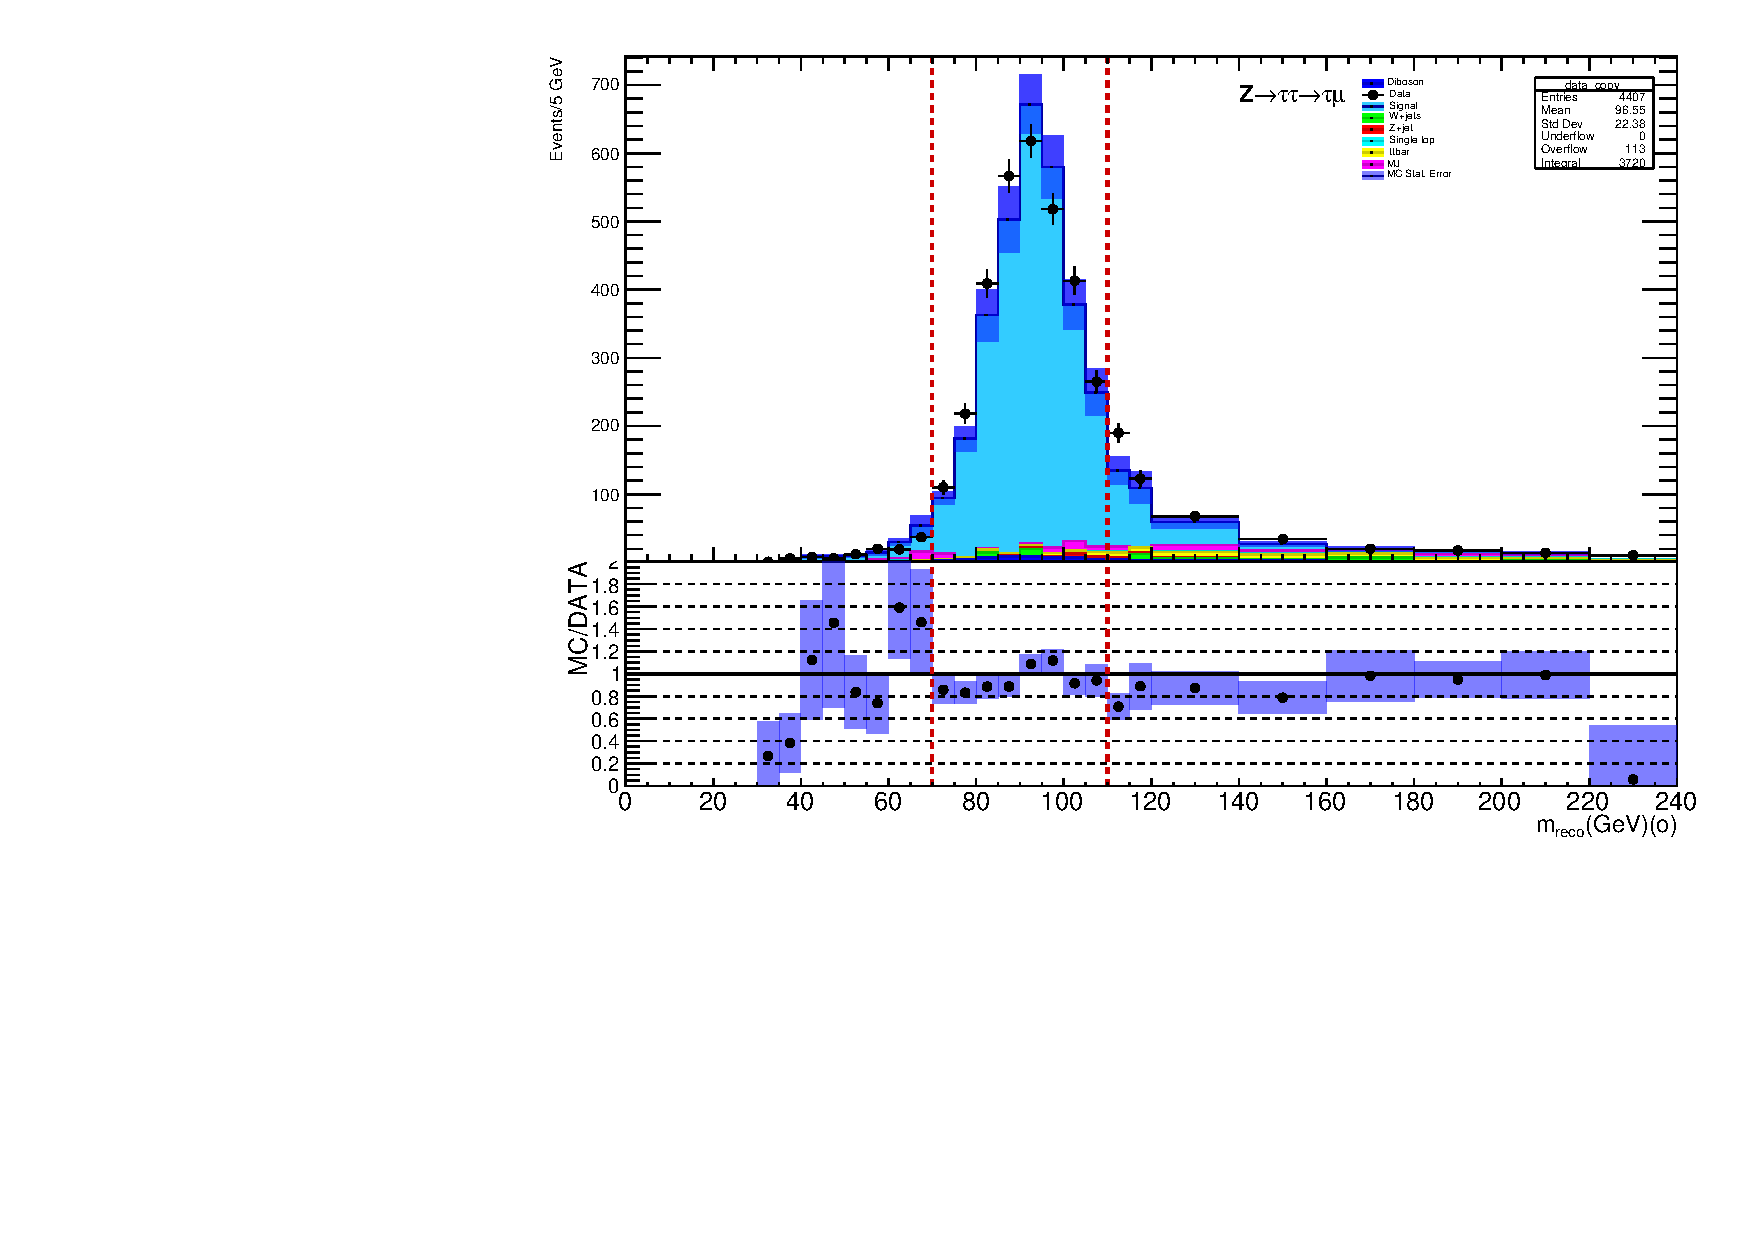
\includegraphics[width=0.50\textwidth]{figures/Fig17g}}}\hfill
	\subfloat[]{\label{Fig17h}{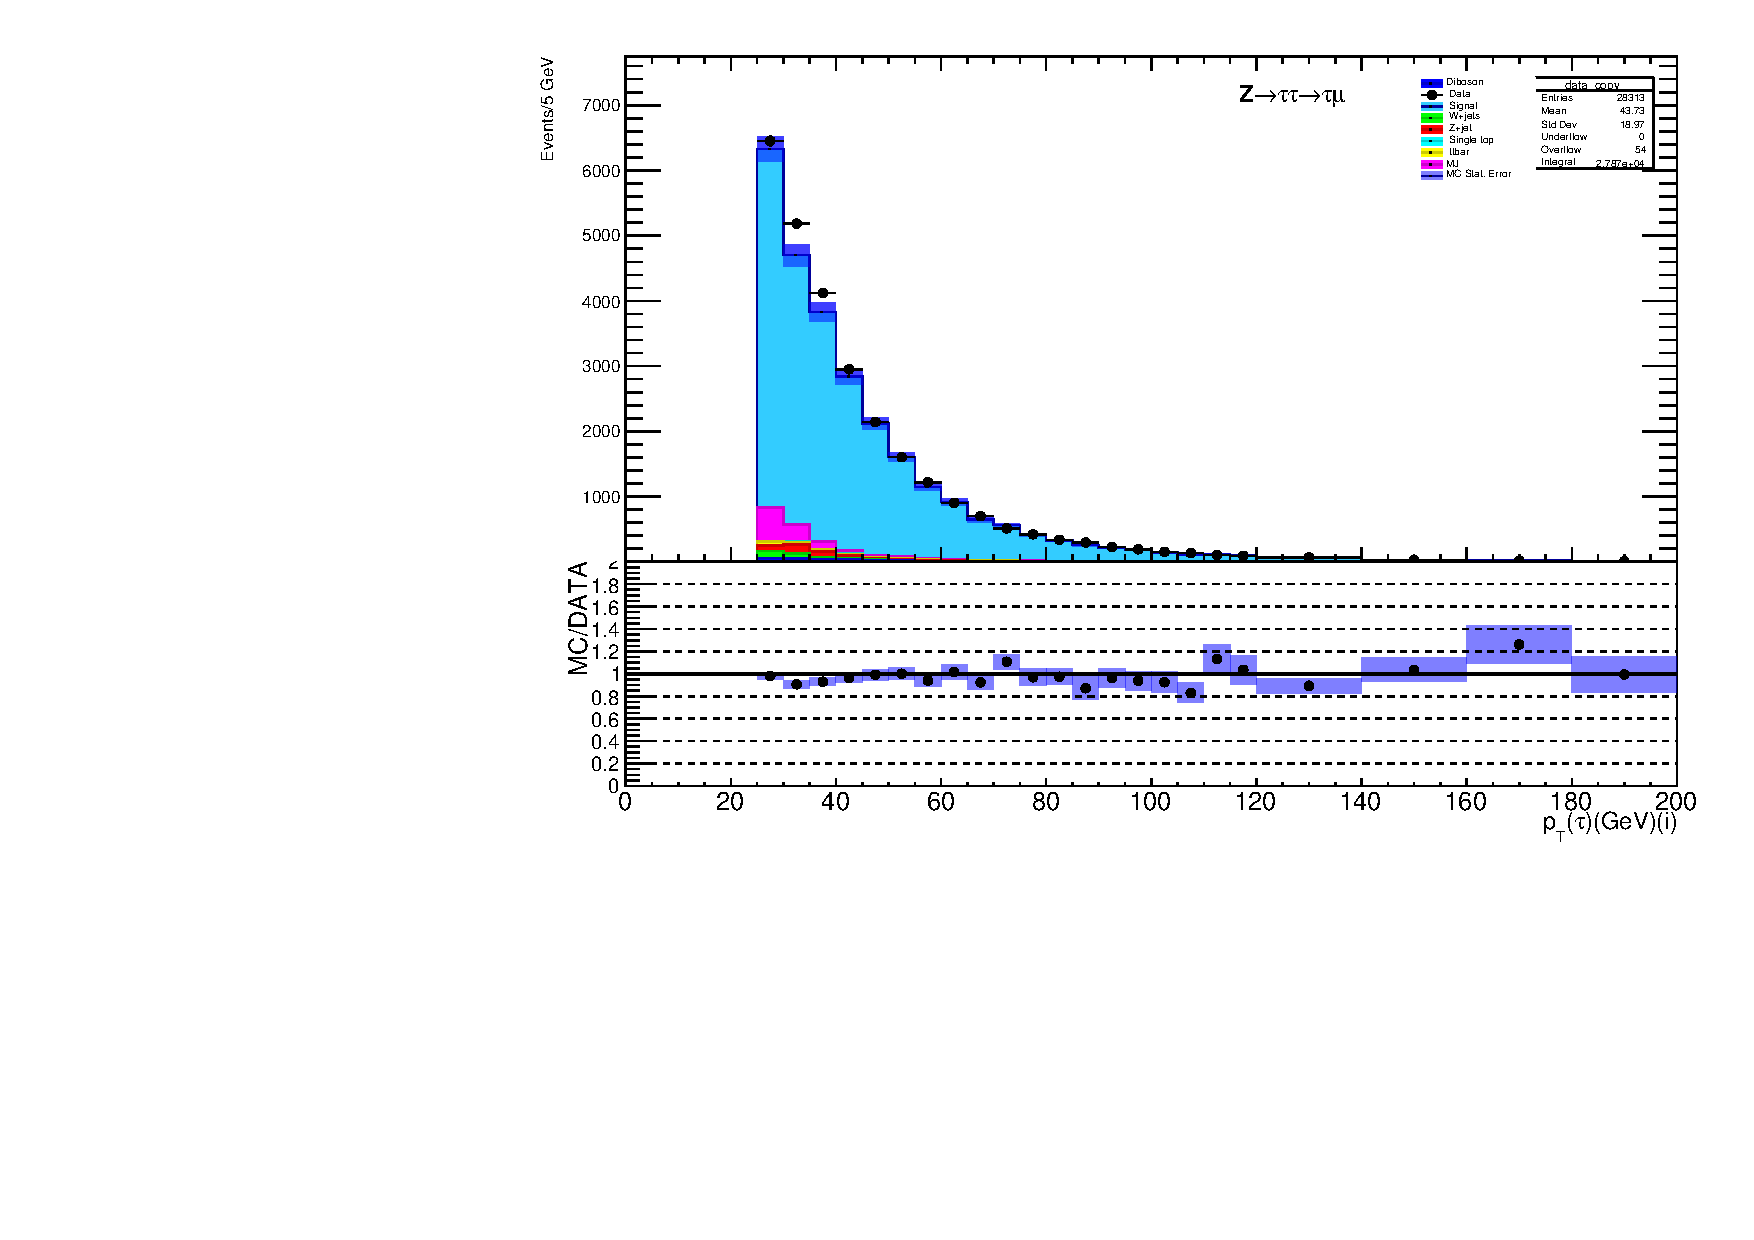
\includegraphics[width=0.50\textwidth]{figures/Fig17h}}}\hfill
	\subfloat[]{\label{Fig17i}{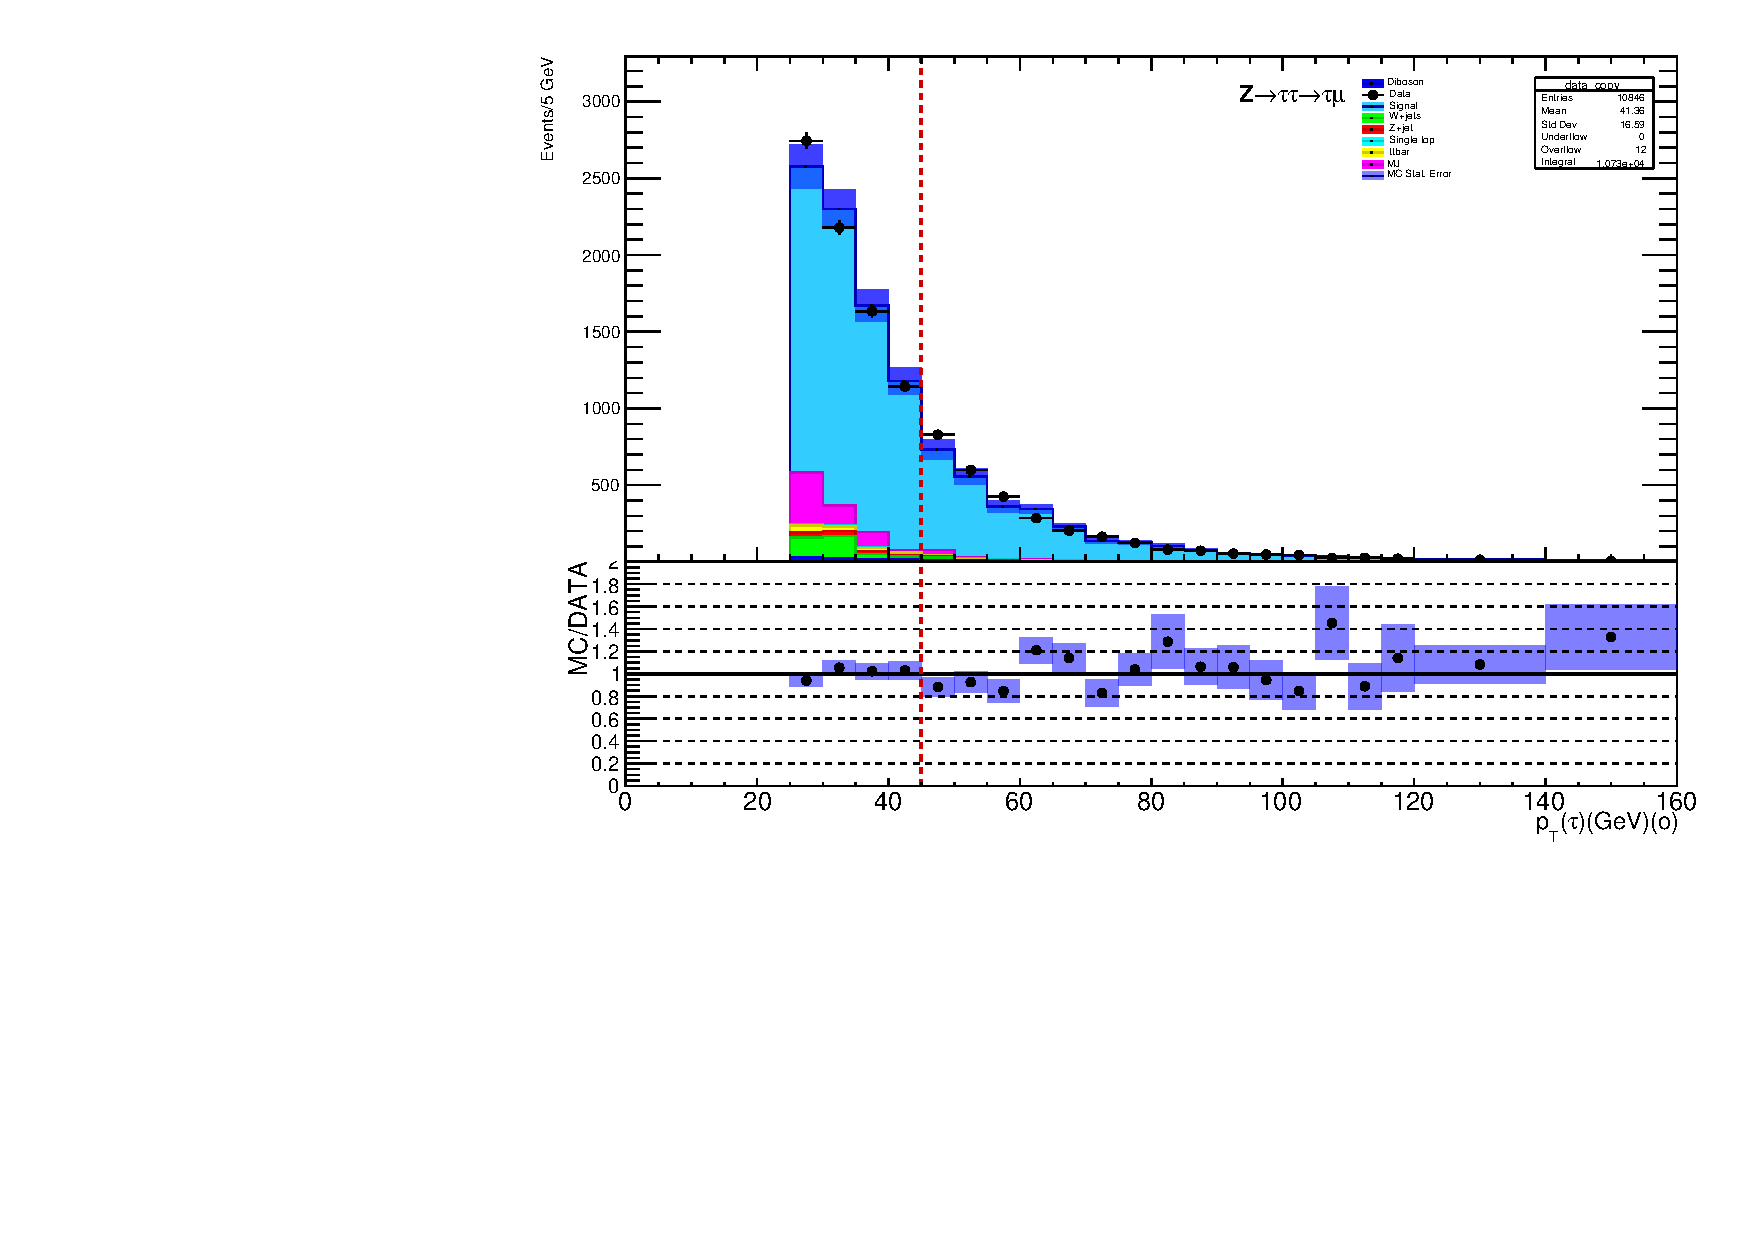
\includegraphics[width=0.50\textwidth]{figures/Fig17i}}}
	\caption{Distributions of all the variables used to select the signal events in the $Z\to\tauh\mu$ final state. In each plot all the cuts have been applied except for the one being displayed. The red vertical bars indicate the value of the cut. The distributions correspond to $\Delta\phi(\tauh,\mu)$ (a), $\pt(\mu)$ (b), RNN score for 1-prong $\tauh$ (c), RNN score for 3-prong $\tauh$ (d), $\Omega$ (e), $\mreco$ for in-between events (f), $\mreco$ for outside events (g), $\pt(\tauh)$ for in-between events (h) and $\pt(\tauh)$ for outside events (i).}
	\label{Fig17}
\end{figure}%
\newpage
\section{$Z\to\tauh e$ final state distributions}

\begin{figure}[H]
	\centering
	\subfloat[]{\label{Fig18a}{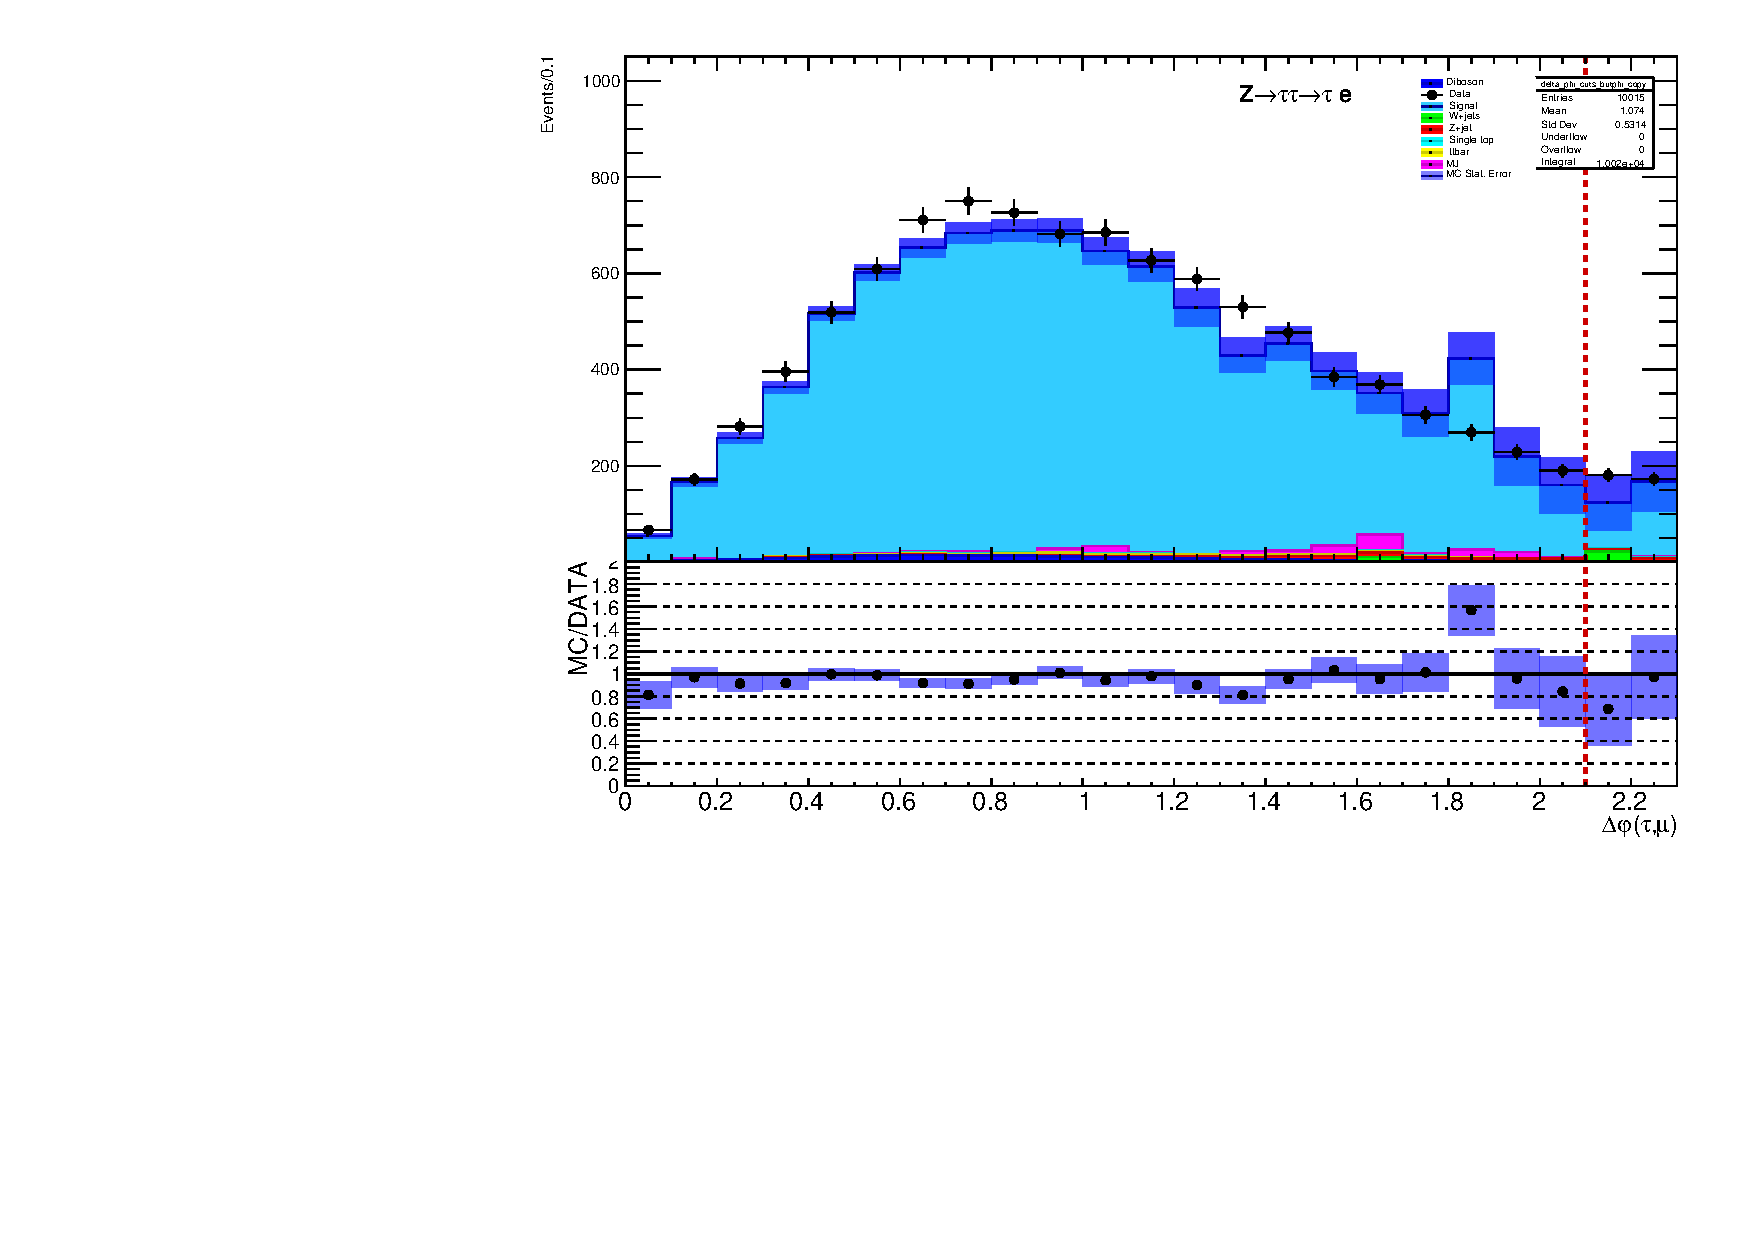
\includegraphics[width=0.50\textwidth]{figures/Fig18a}}}\hfill
	\subfloat[]{\label{Fig18b}{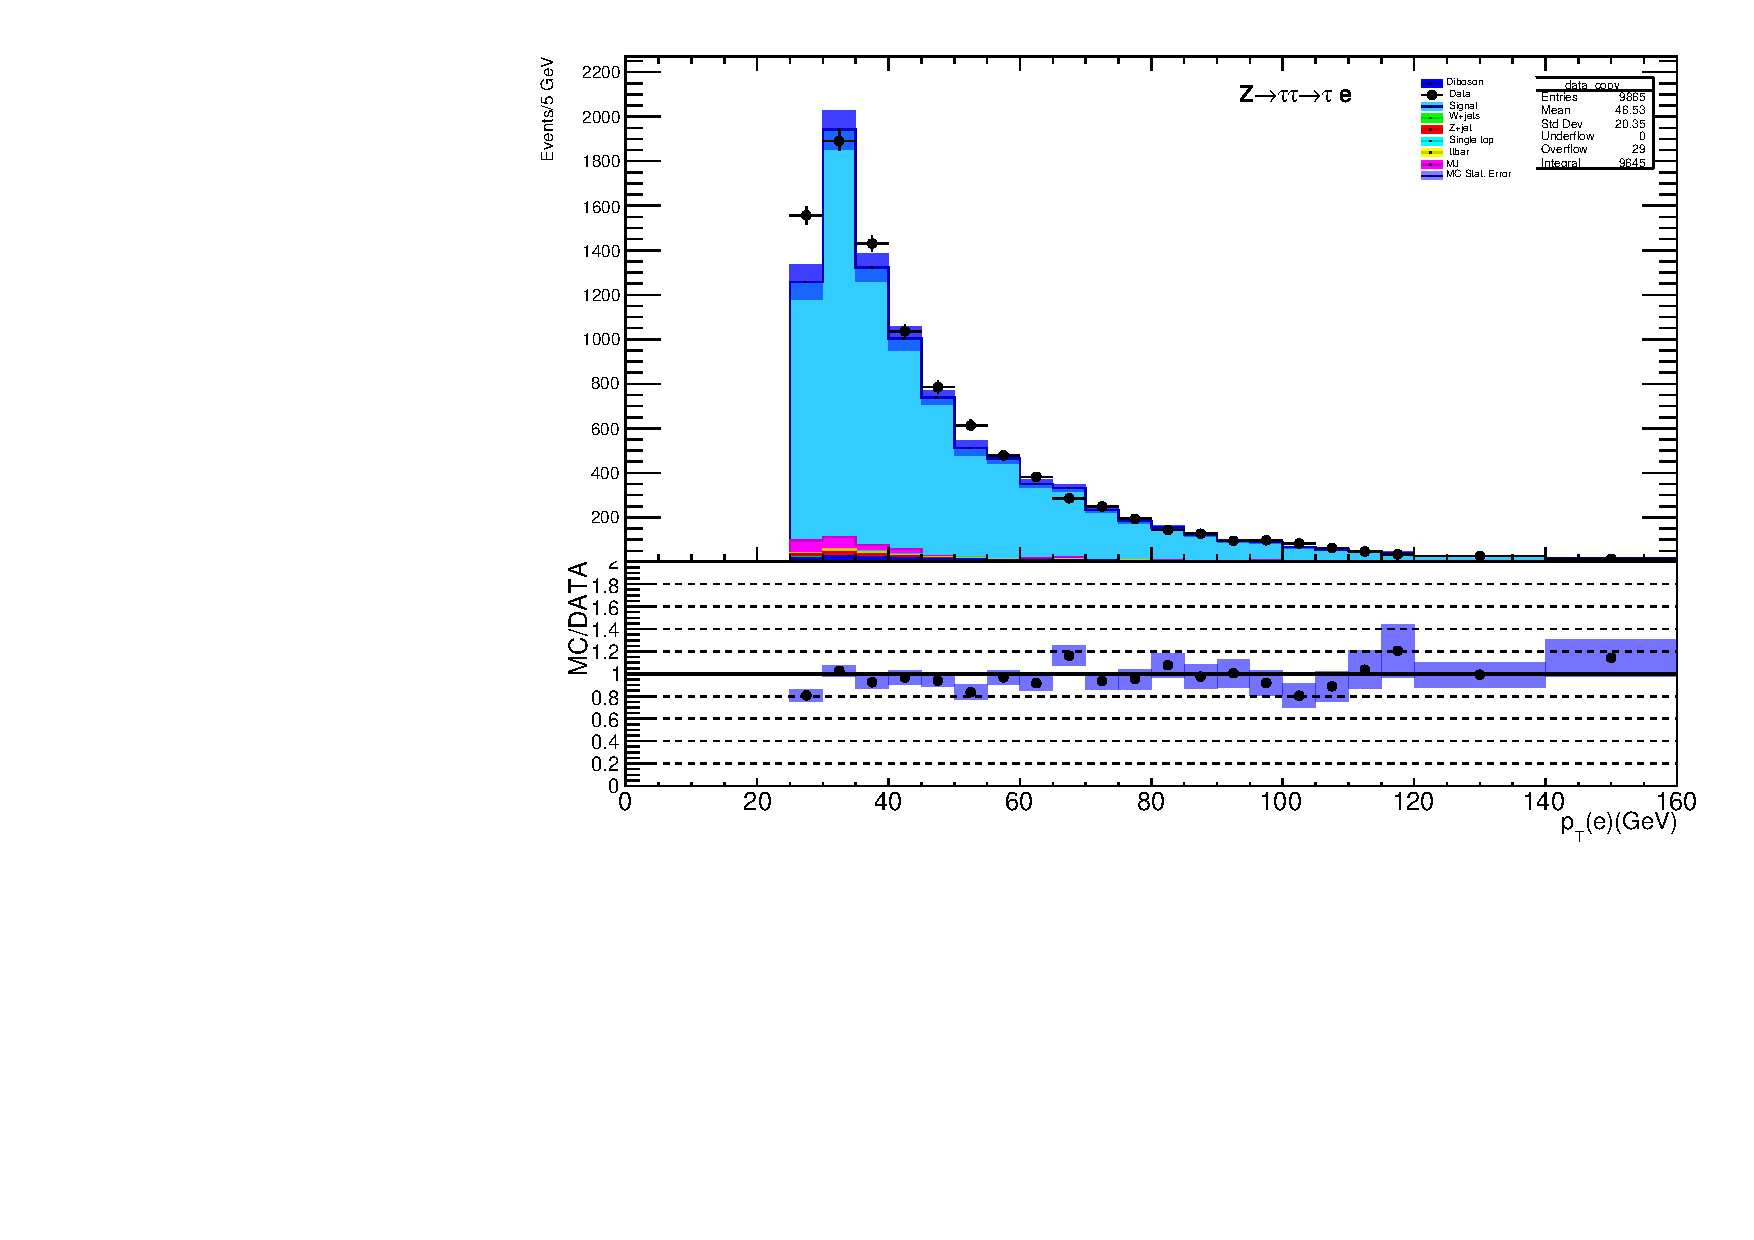
\includegraphics[width=0.50\textwidth]{figures/Fig18b}}}\hfill
	\subfloat[]{\label{Fig18c}{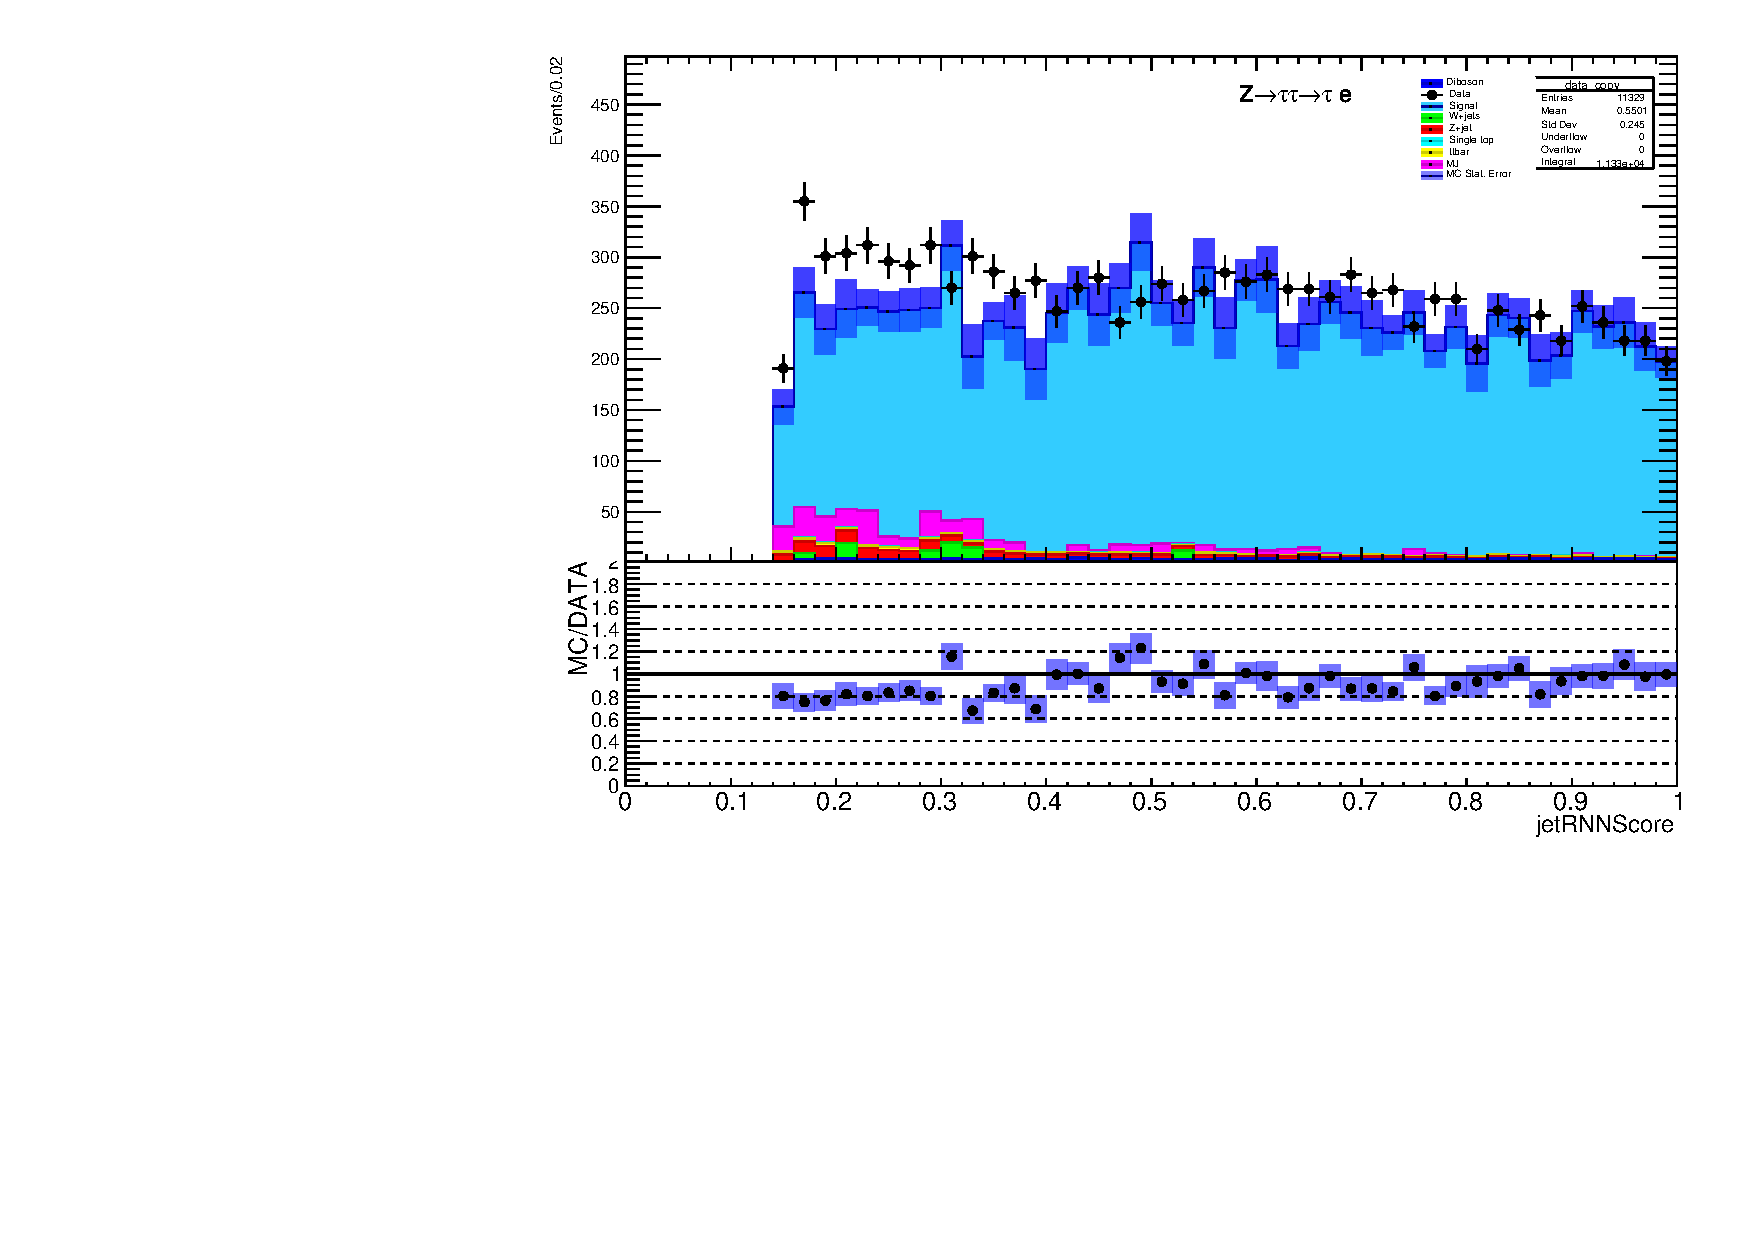
\includegraphics[width=0.50\textwidth]{figures/Fig18c}}}\hfill
	\subfloat[]{\label{Fig18d}{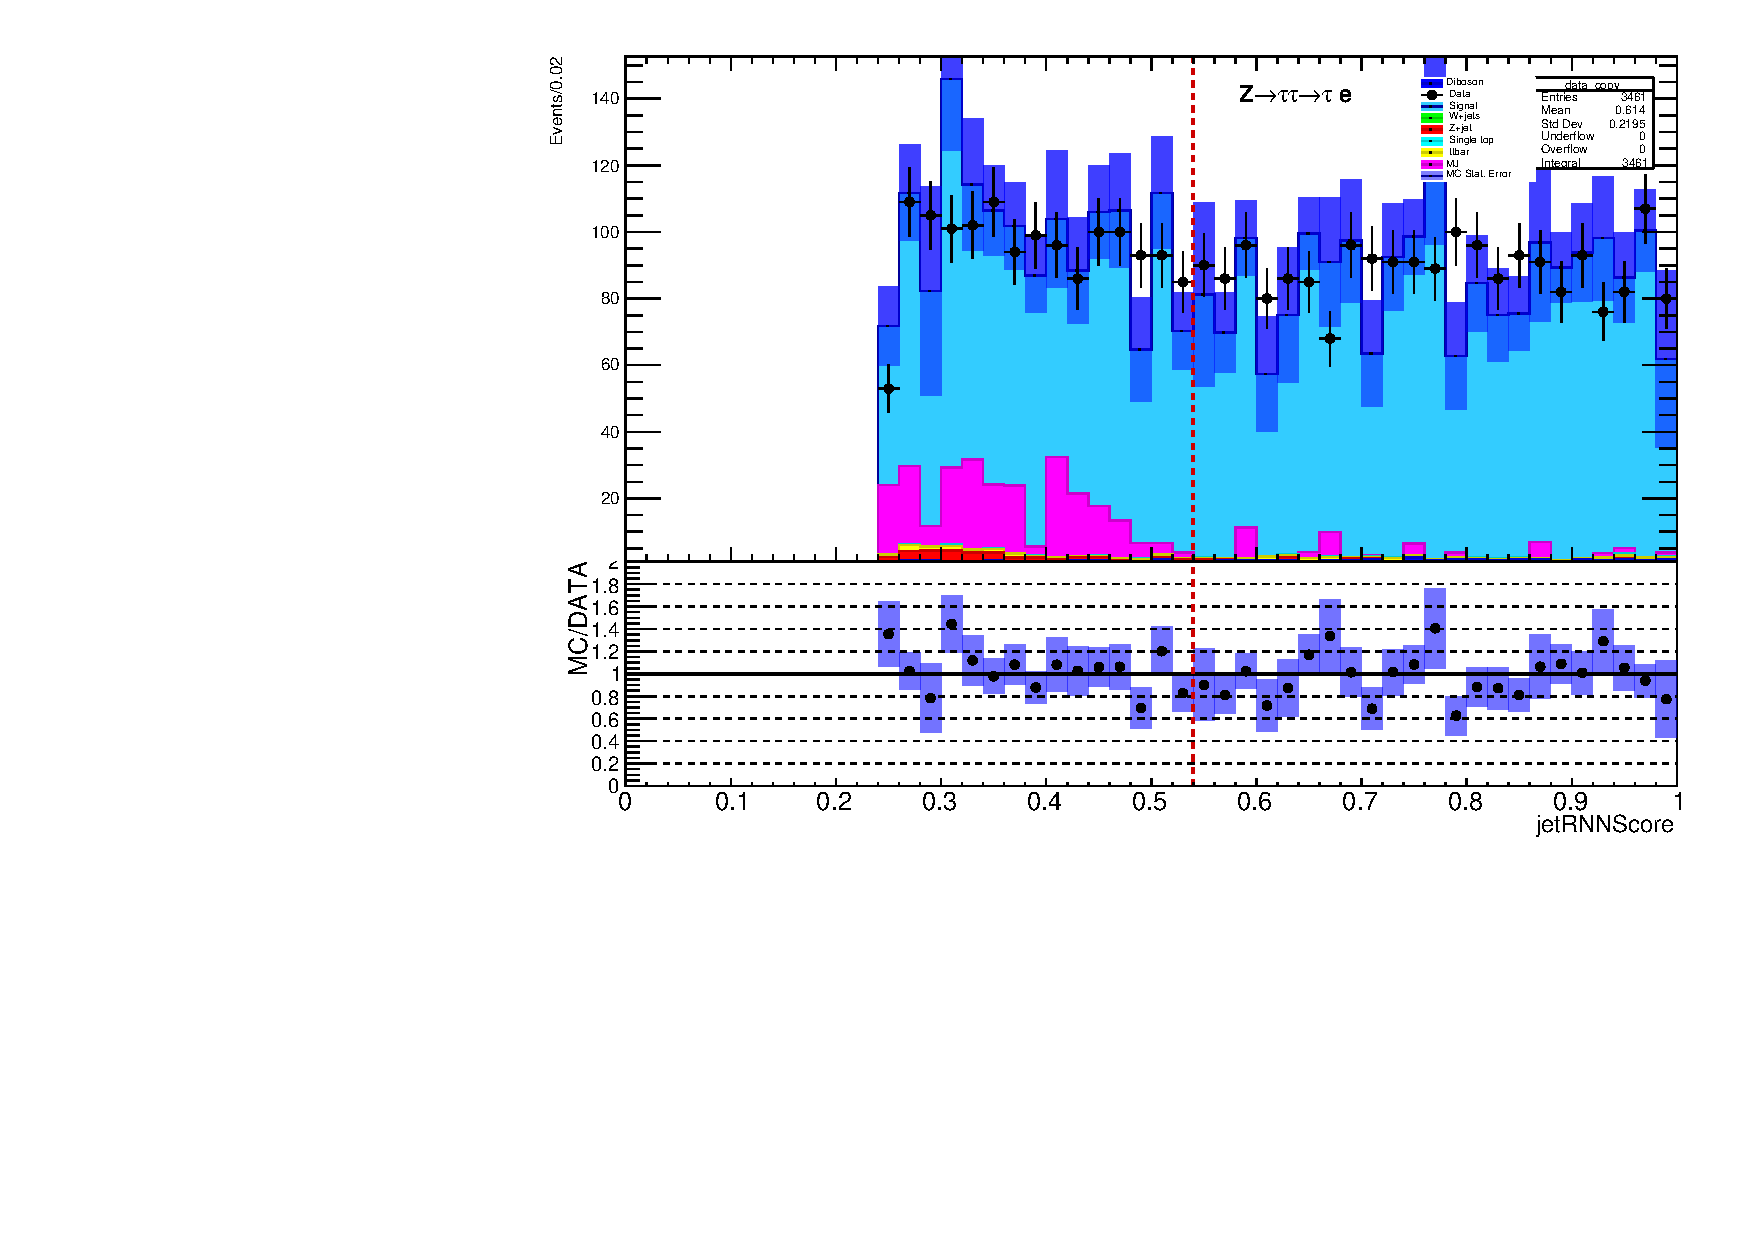
\includegraphics[width=0.50\textwidth]{figures/Fig18d}}}\hfill
	\subfloat[]{\label{Fig18e}{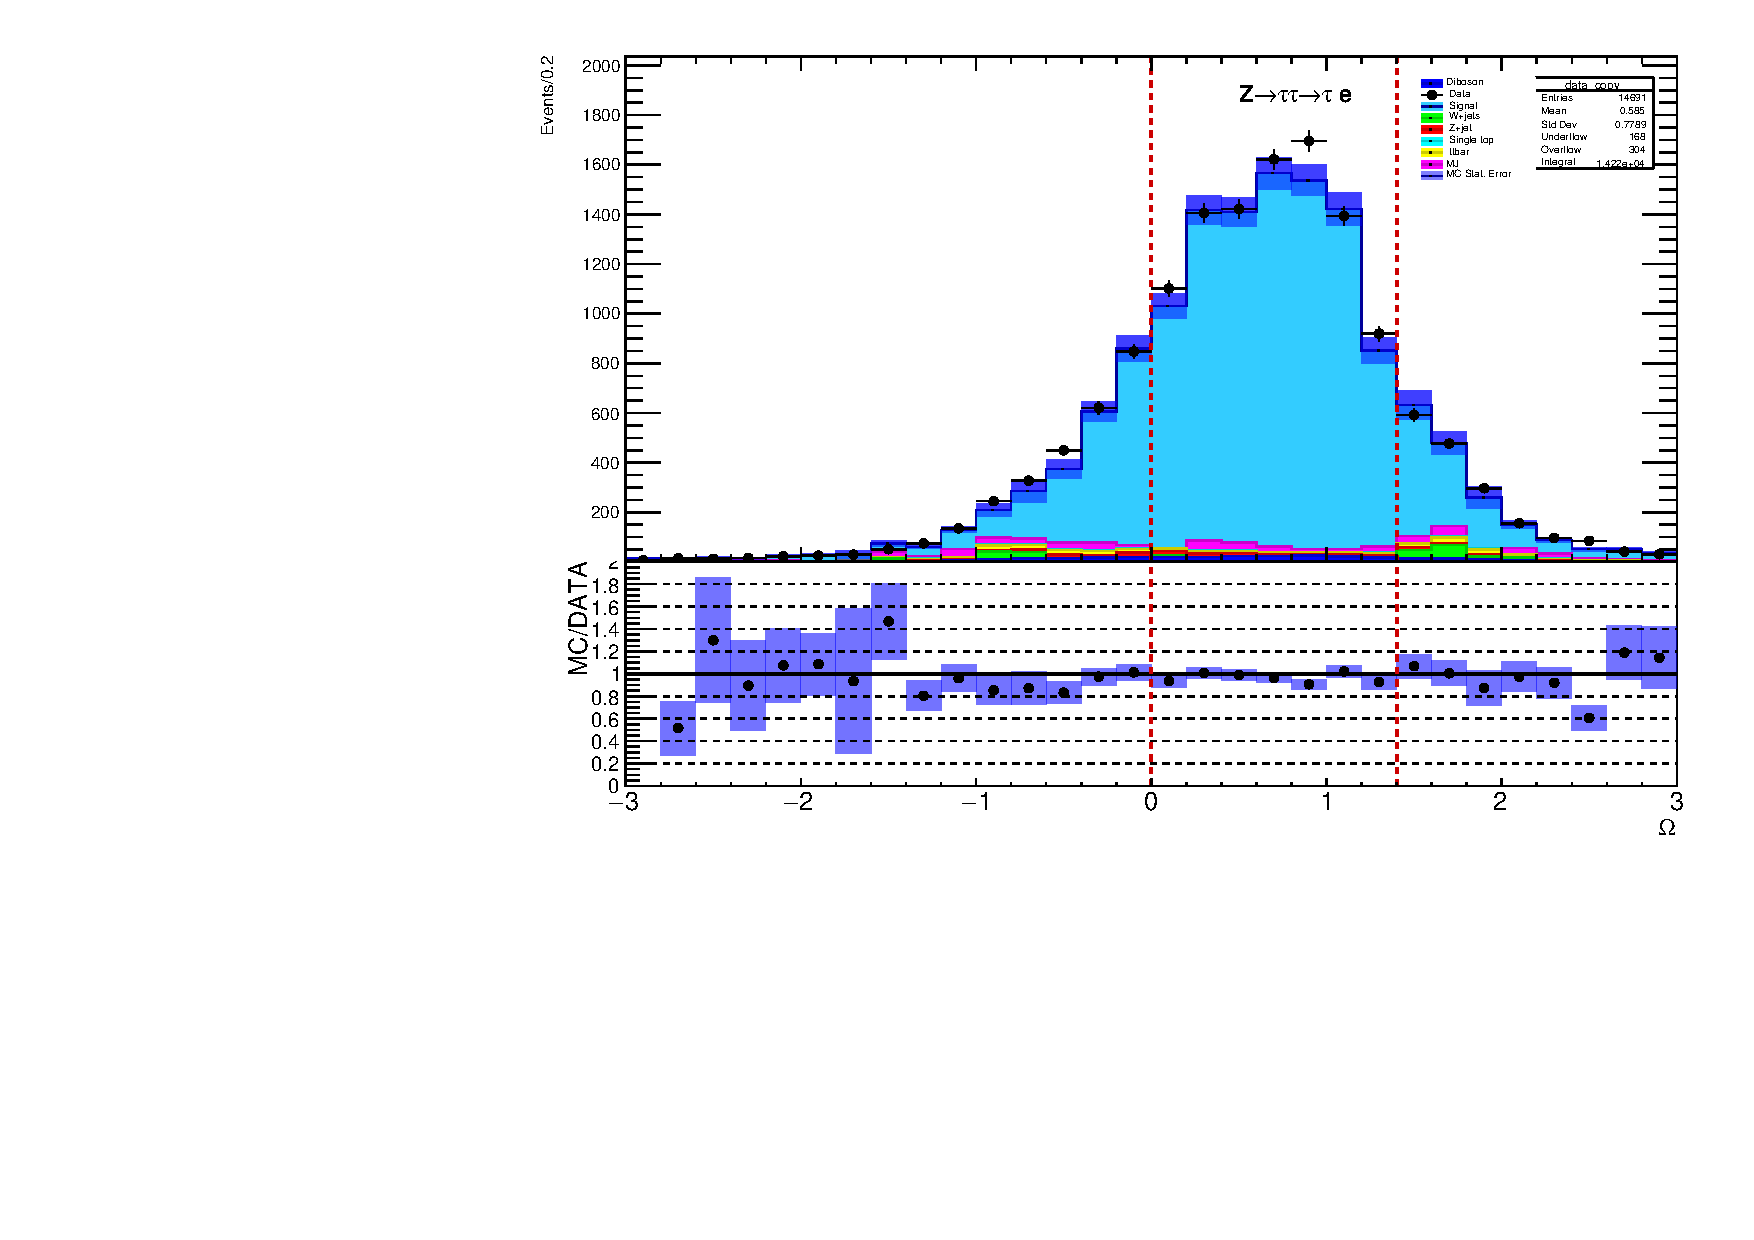
\includegraphics[width=0.50\textwidth]{figures/Fig18e}}}\hfill
	\subfloat[]{\label{Fig18f}{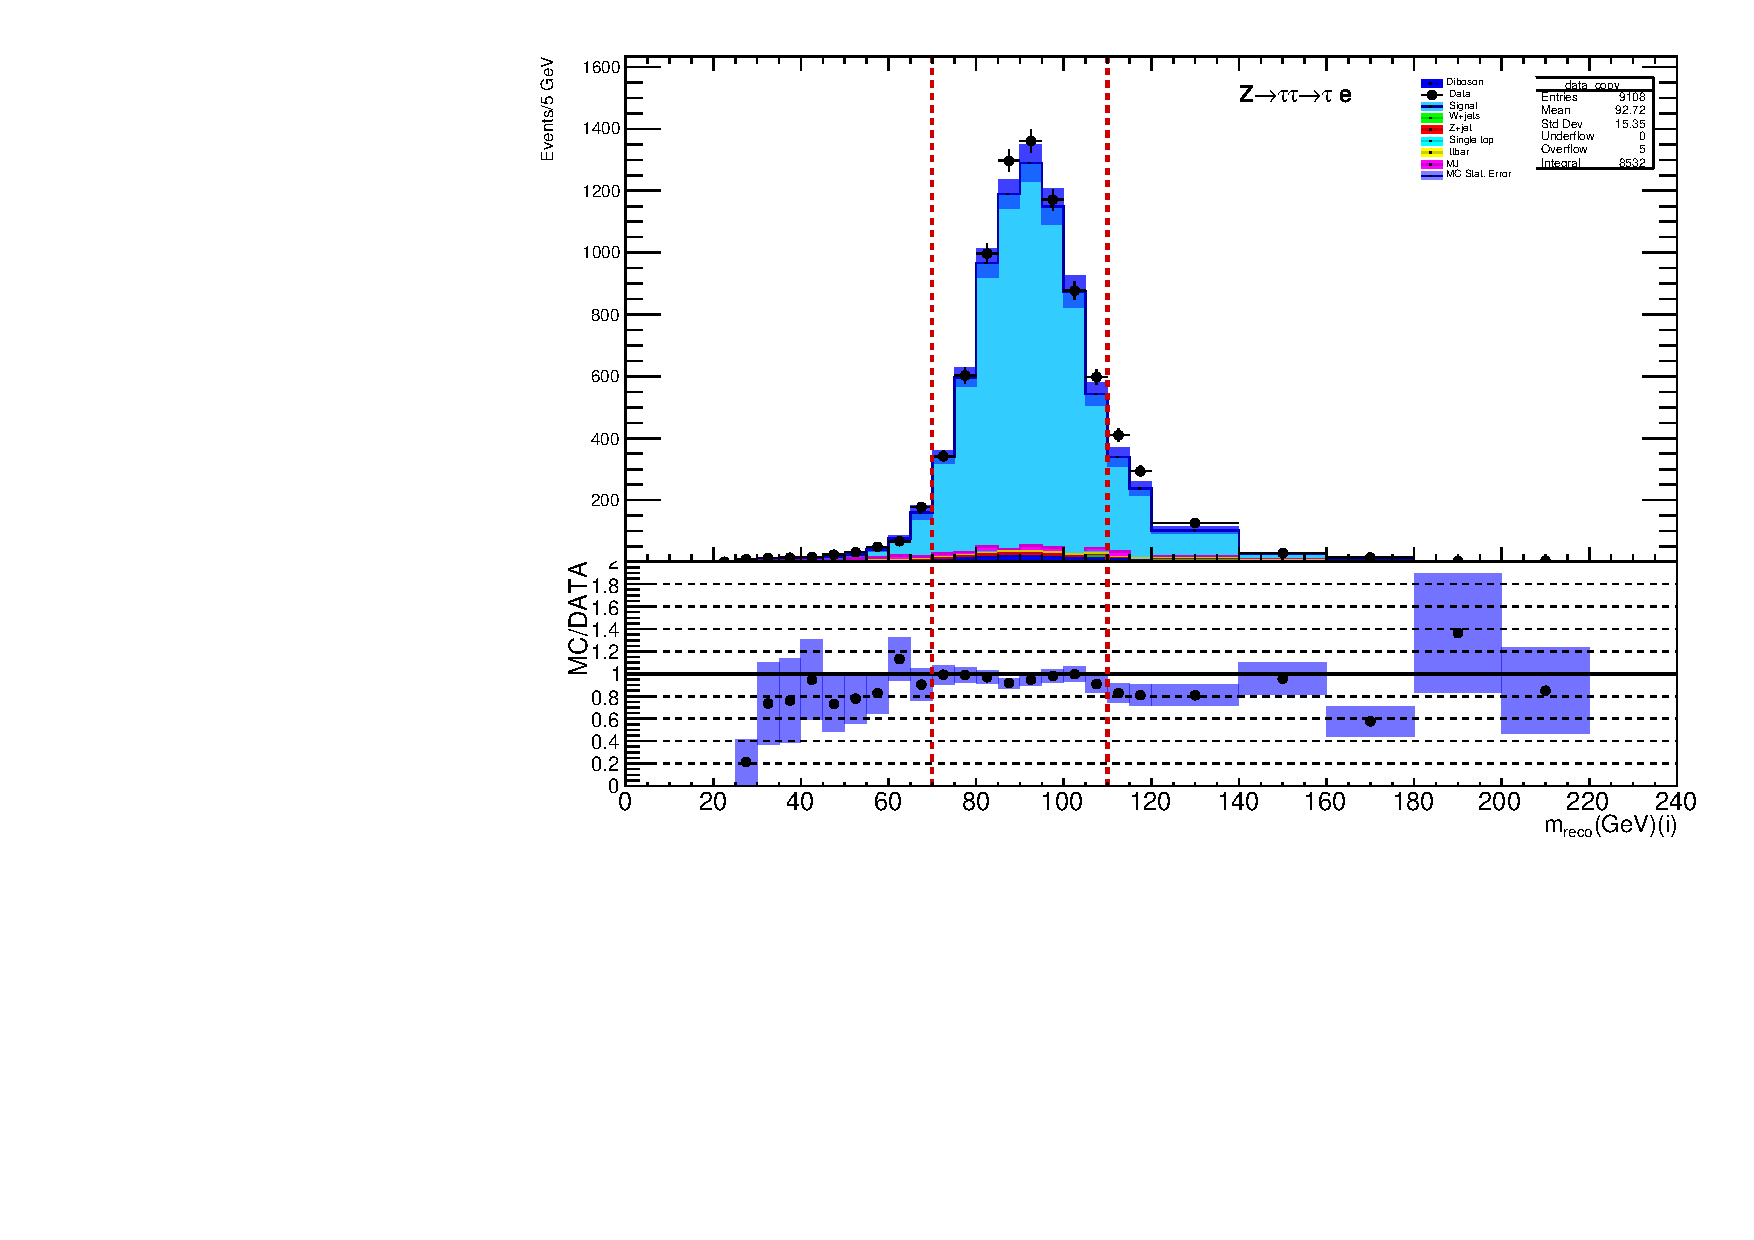
\includegraphics[width=0.50\textwidth]{figures/Fig18f}}}
	\label{Fig18}
\end{figure}
\begin{figure}[H]\ContinuedFloat
	\centering
	\subfloat[]{\label{Fig18g}{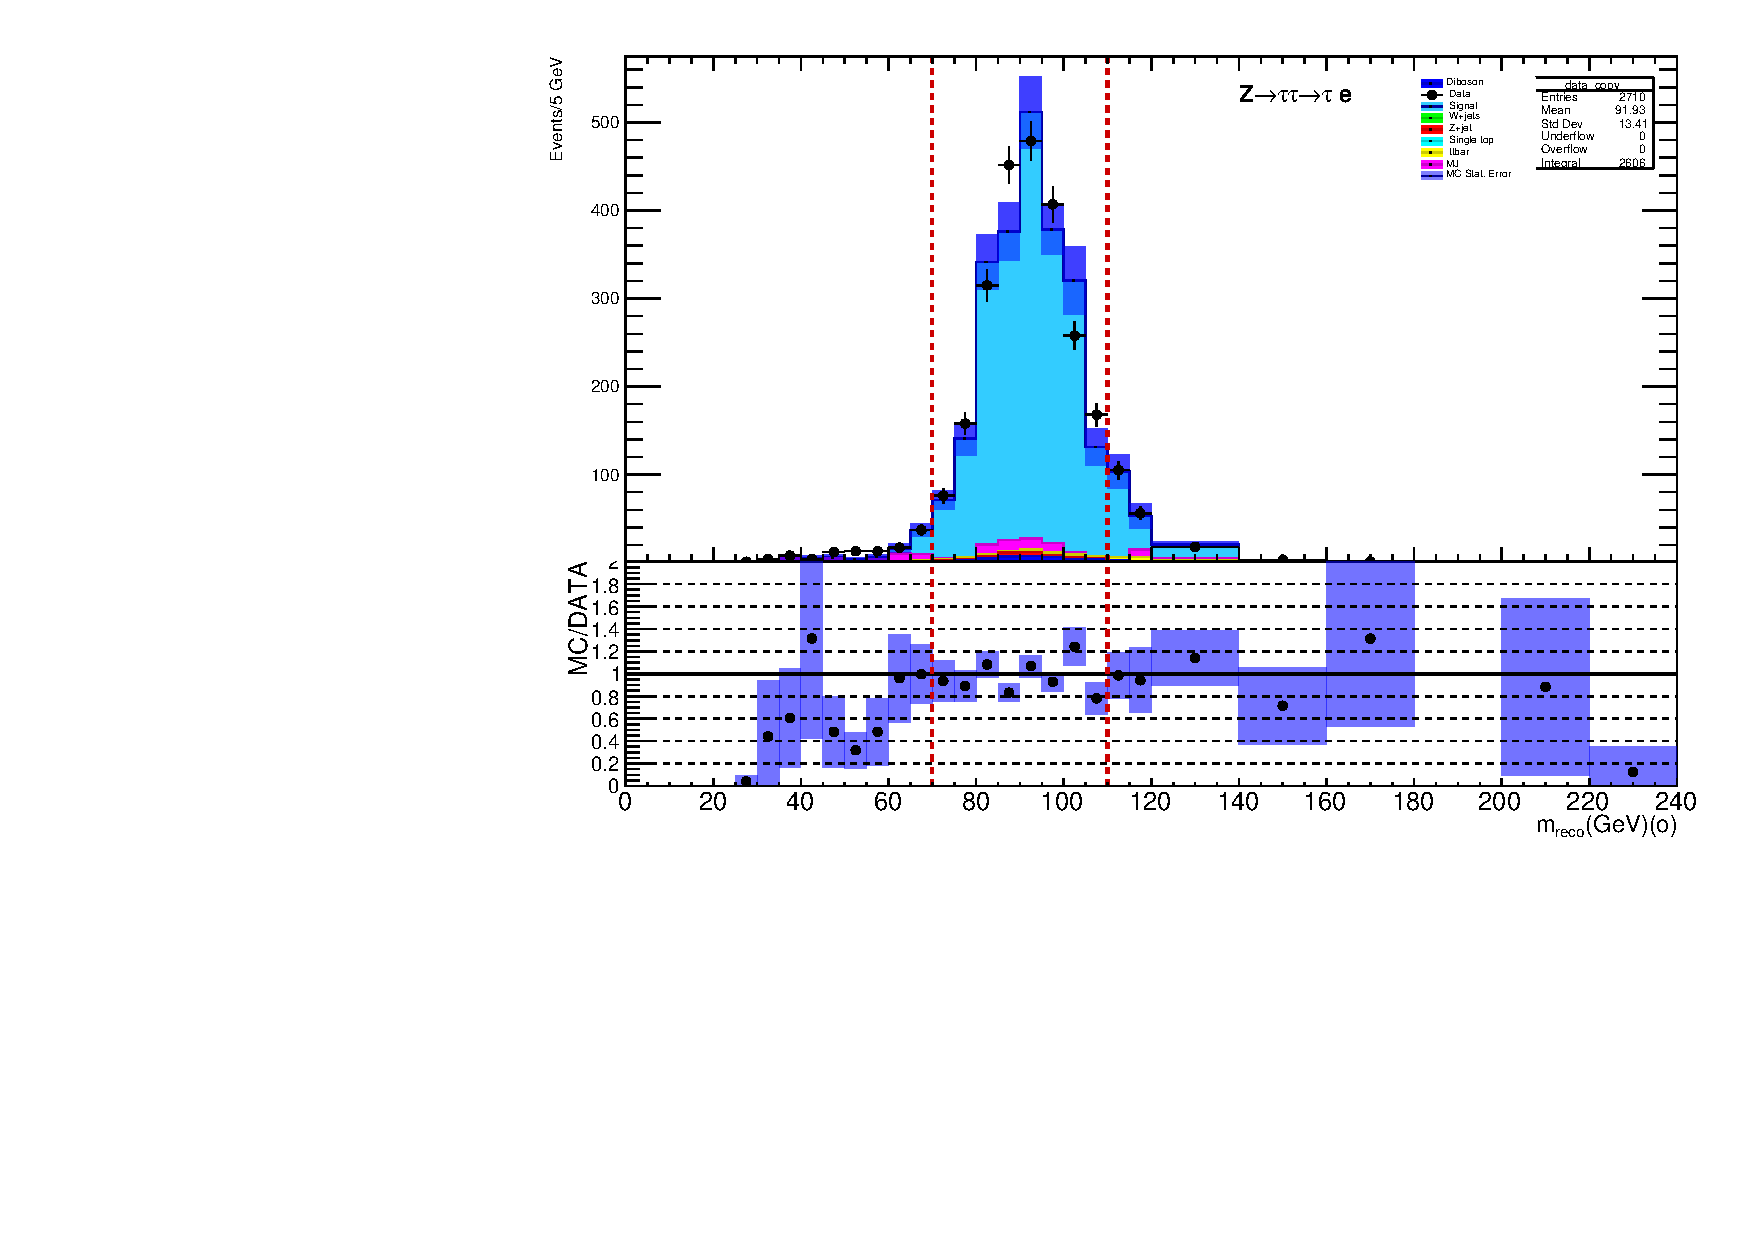
\includegraphics[width=0.50\textwidth]{figures/Fig18g}}}\hfill
	\subfloat[]{\label{Fig18h}{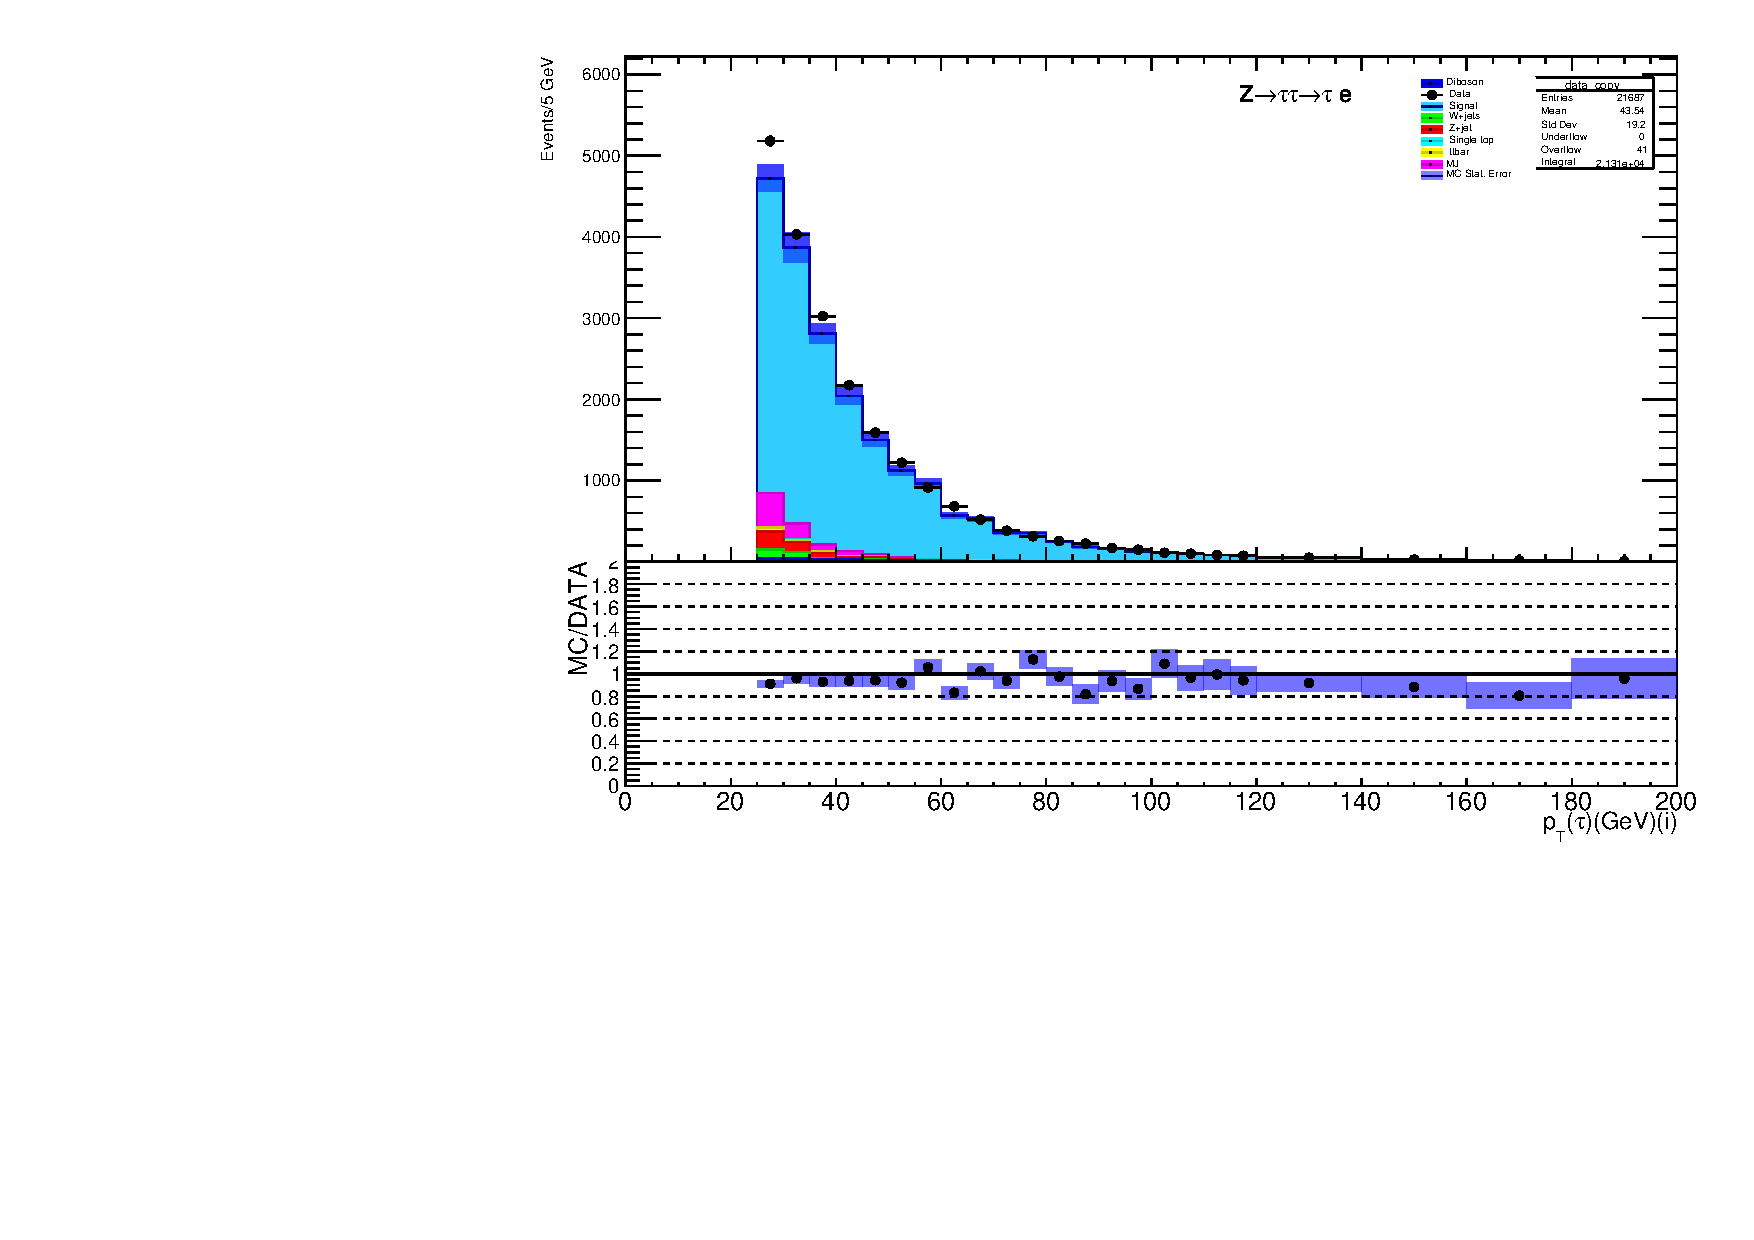
\includegraphics[width=0.50\textwidth]{figures/Fig18h}}}\hfill
	\subfloat[]{\label{Fig18i}{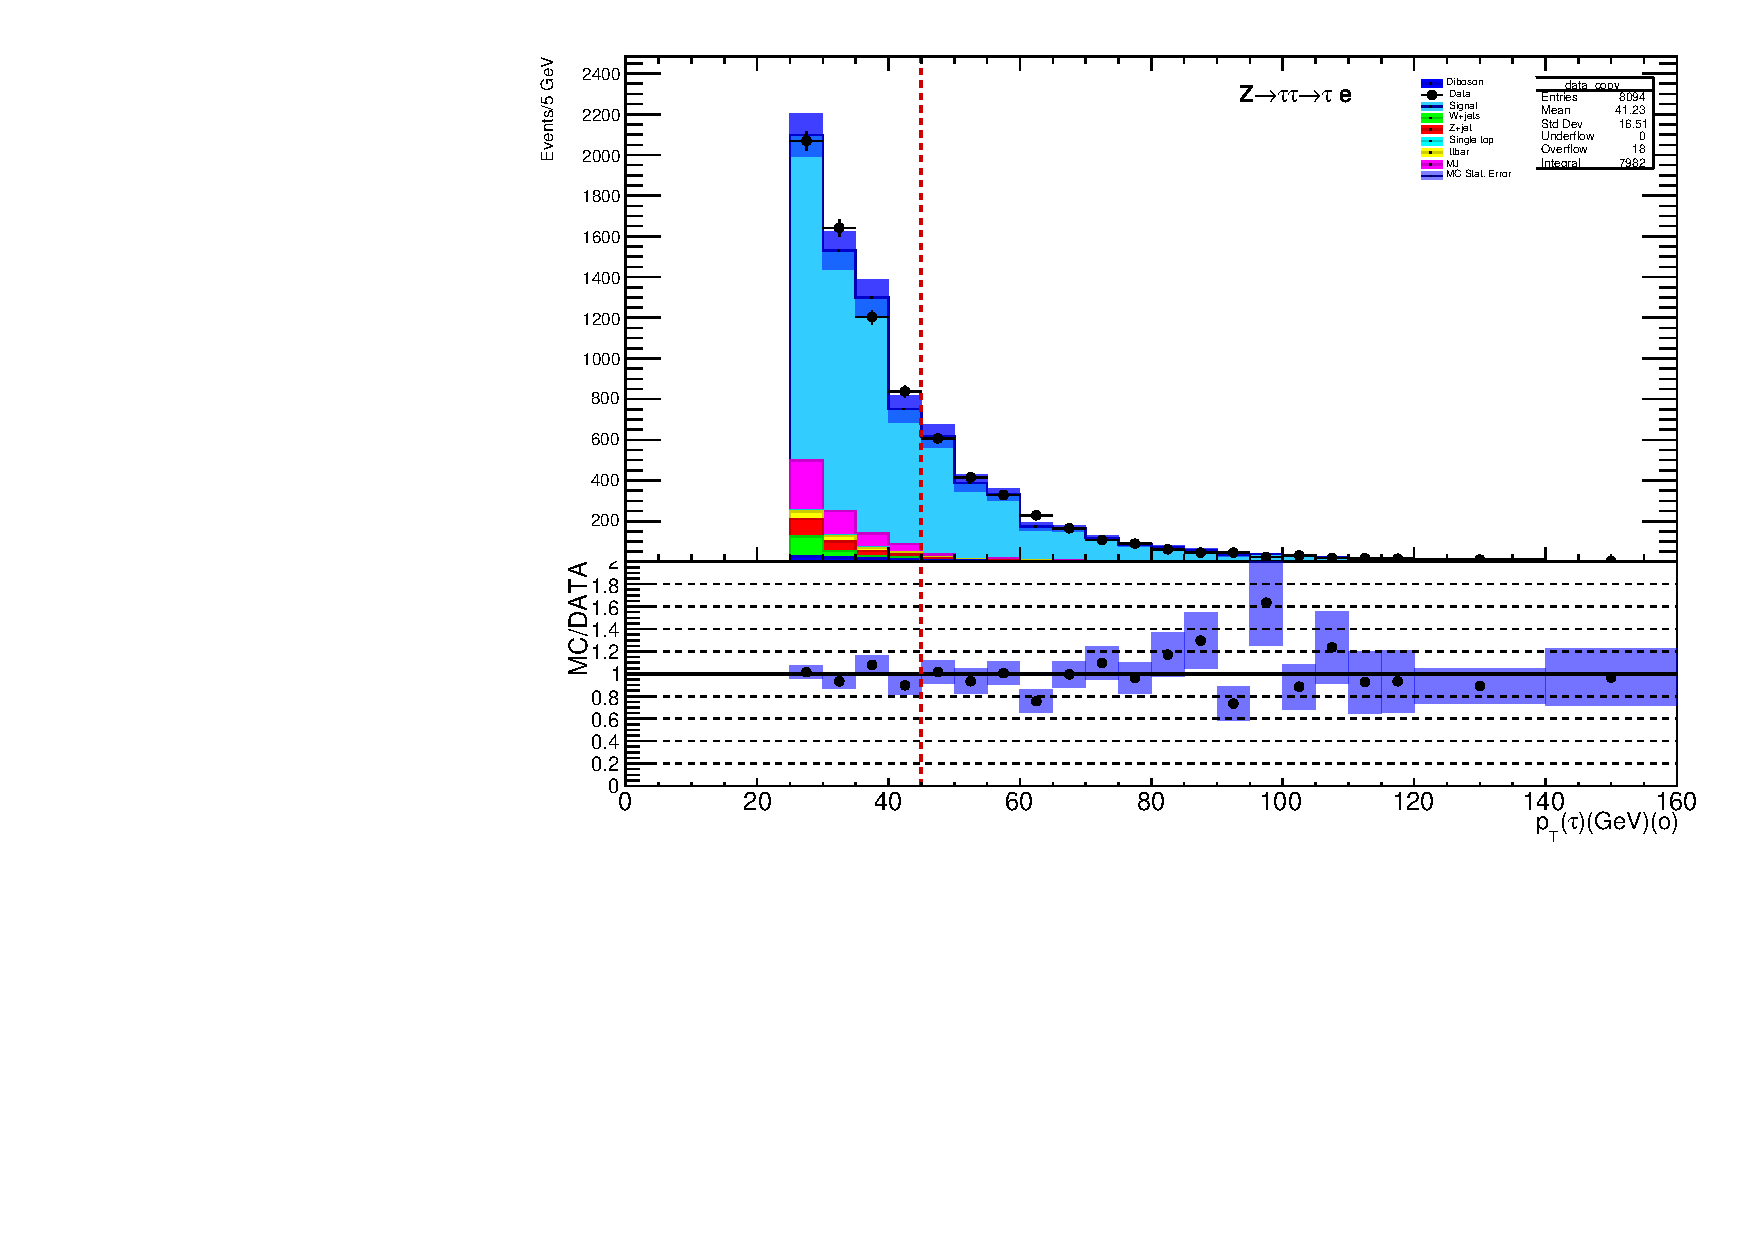
\includegraphics[width=0.50\textwidth]{figures/Fig18i}}}\hfill
	\subfloat[]{\label{Fig18j}{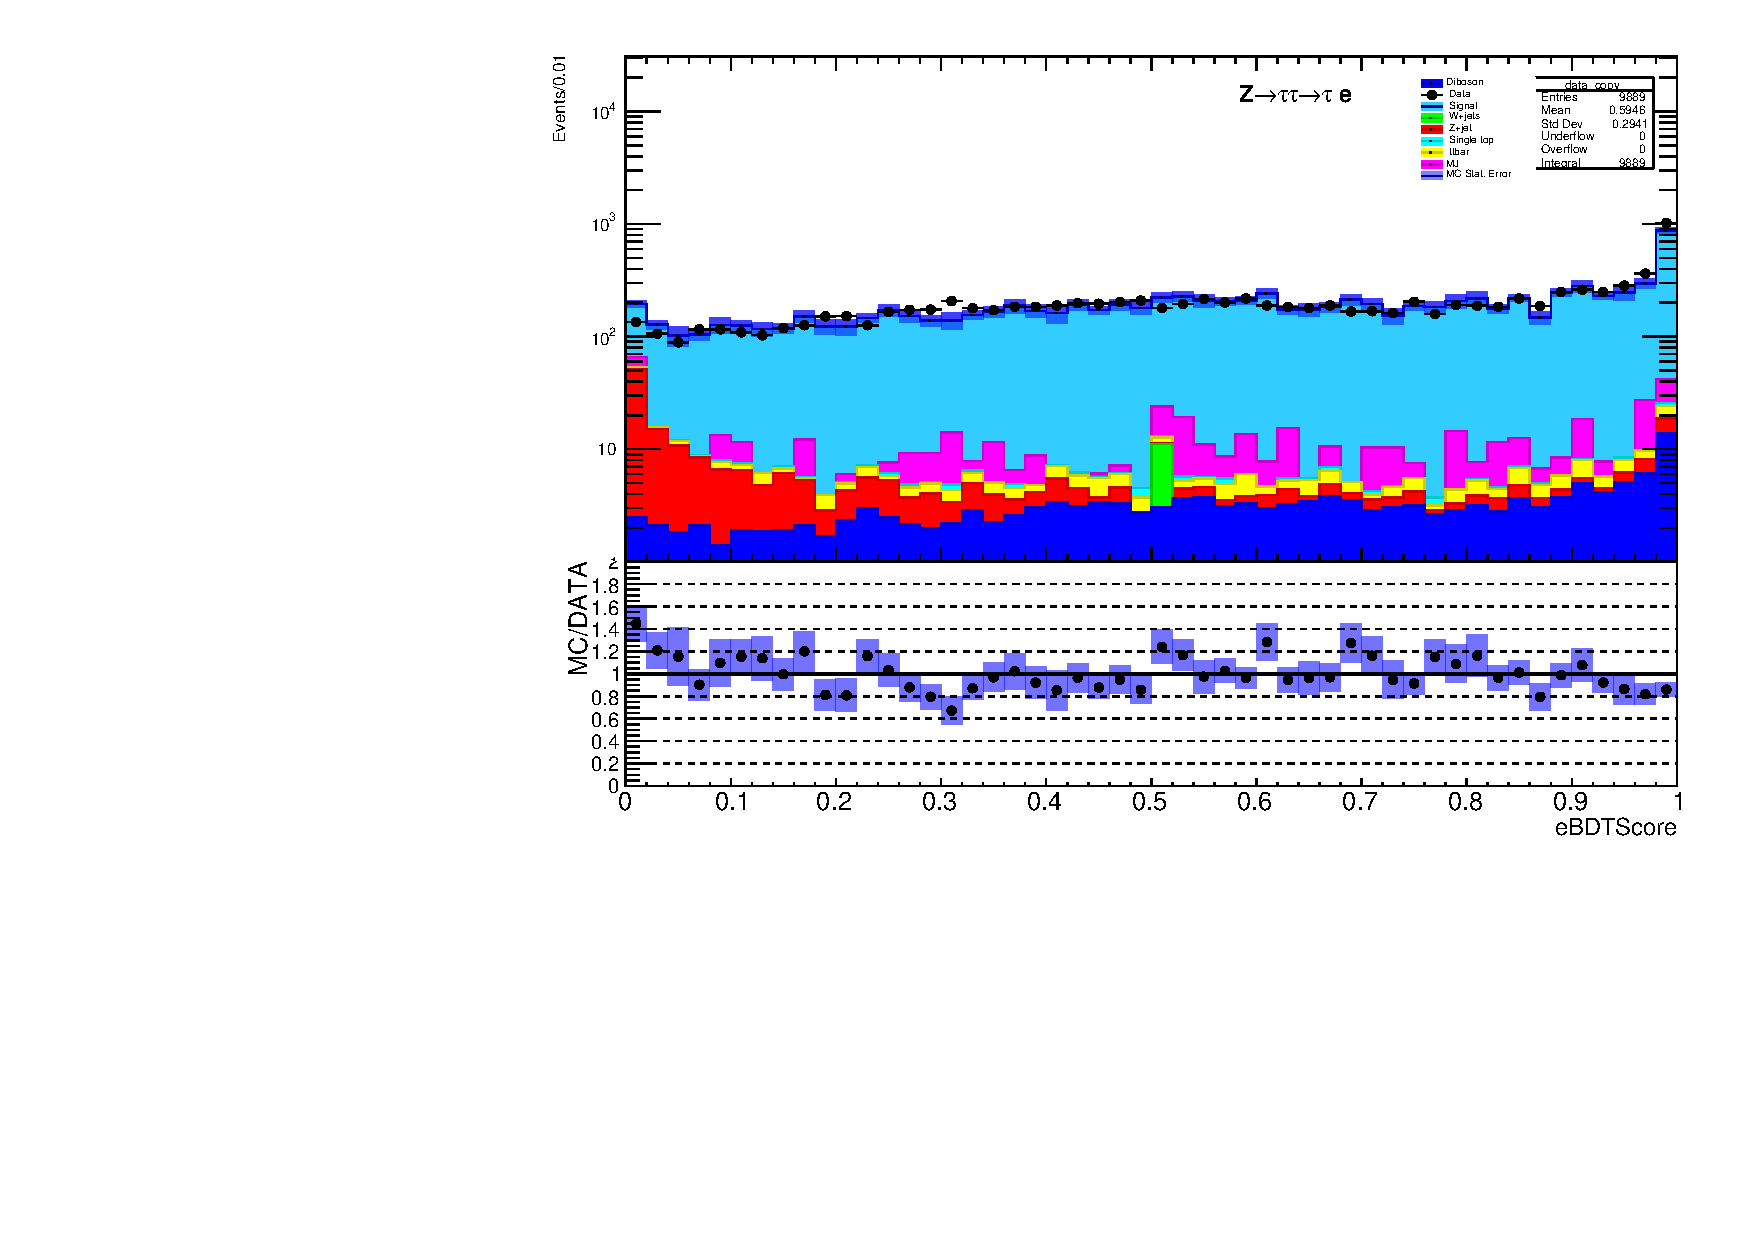
\includegraphics[width=0.50\textwidth]{figures/Fig18j}}}\hfill
	\subfloat[]{\label{Fig18k}{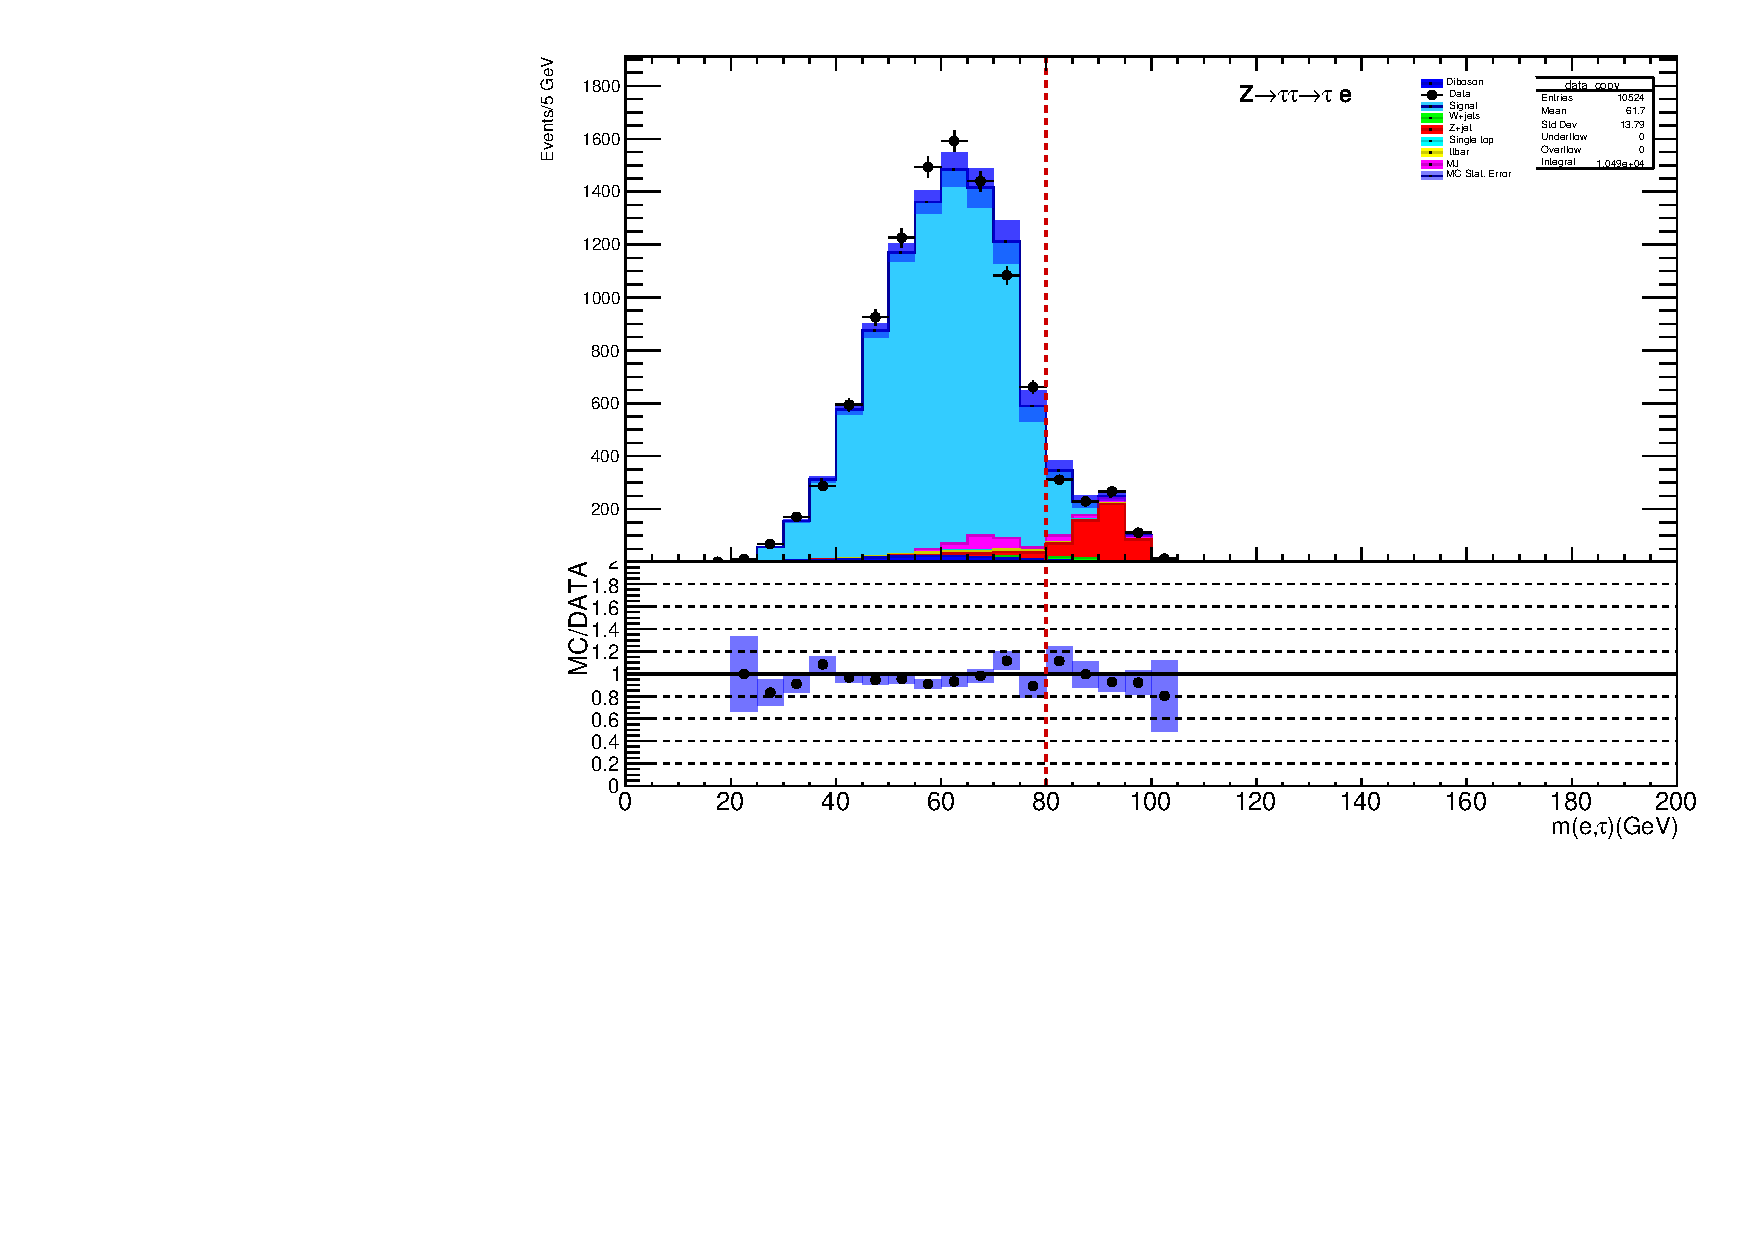
\includegraphics[width=0.50\textwidth]{figures/Fig18k}}}
	\caption{Distributions of all the variables used to select the signal events in the $Z\to\tauh e$ final state. In each plot all the cuts have been applied except for the one being displayed. The red vertical bars indicate the value of the cut. The distributions correspond to $\Delta\phi(\tauh,e)$ (a), $\pt(e)$ (b), RNN score for 1-prong $\tauh$ (c), RNN score for 3-prong $\tauh$ (d), $\Omega$ (e), $\mreco$ for in-between events (f), $\mreco$ for outside events (g), $\pt(\tauh)$ for in-between events (h), $\pt(\tauh)$ for outside events (i), electron BDT score (j) and $m(\tauh,e)$ (k).}
	\label{Fig18}
\end{figure}
\section{Z$\pt$ distributions}
\begin{figure}[H]
	\centering
	\subfloat[]{\label{Fig21a}{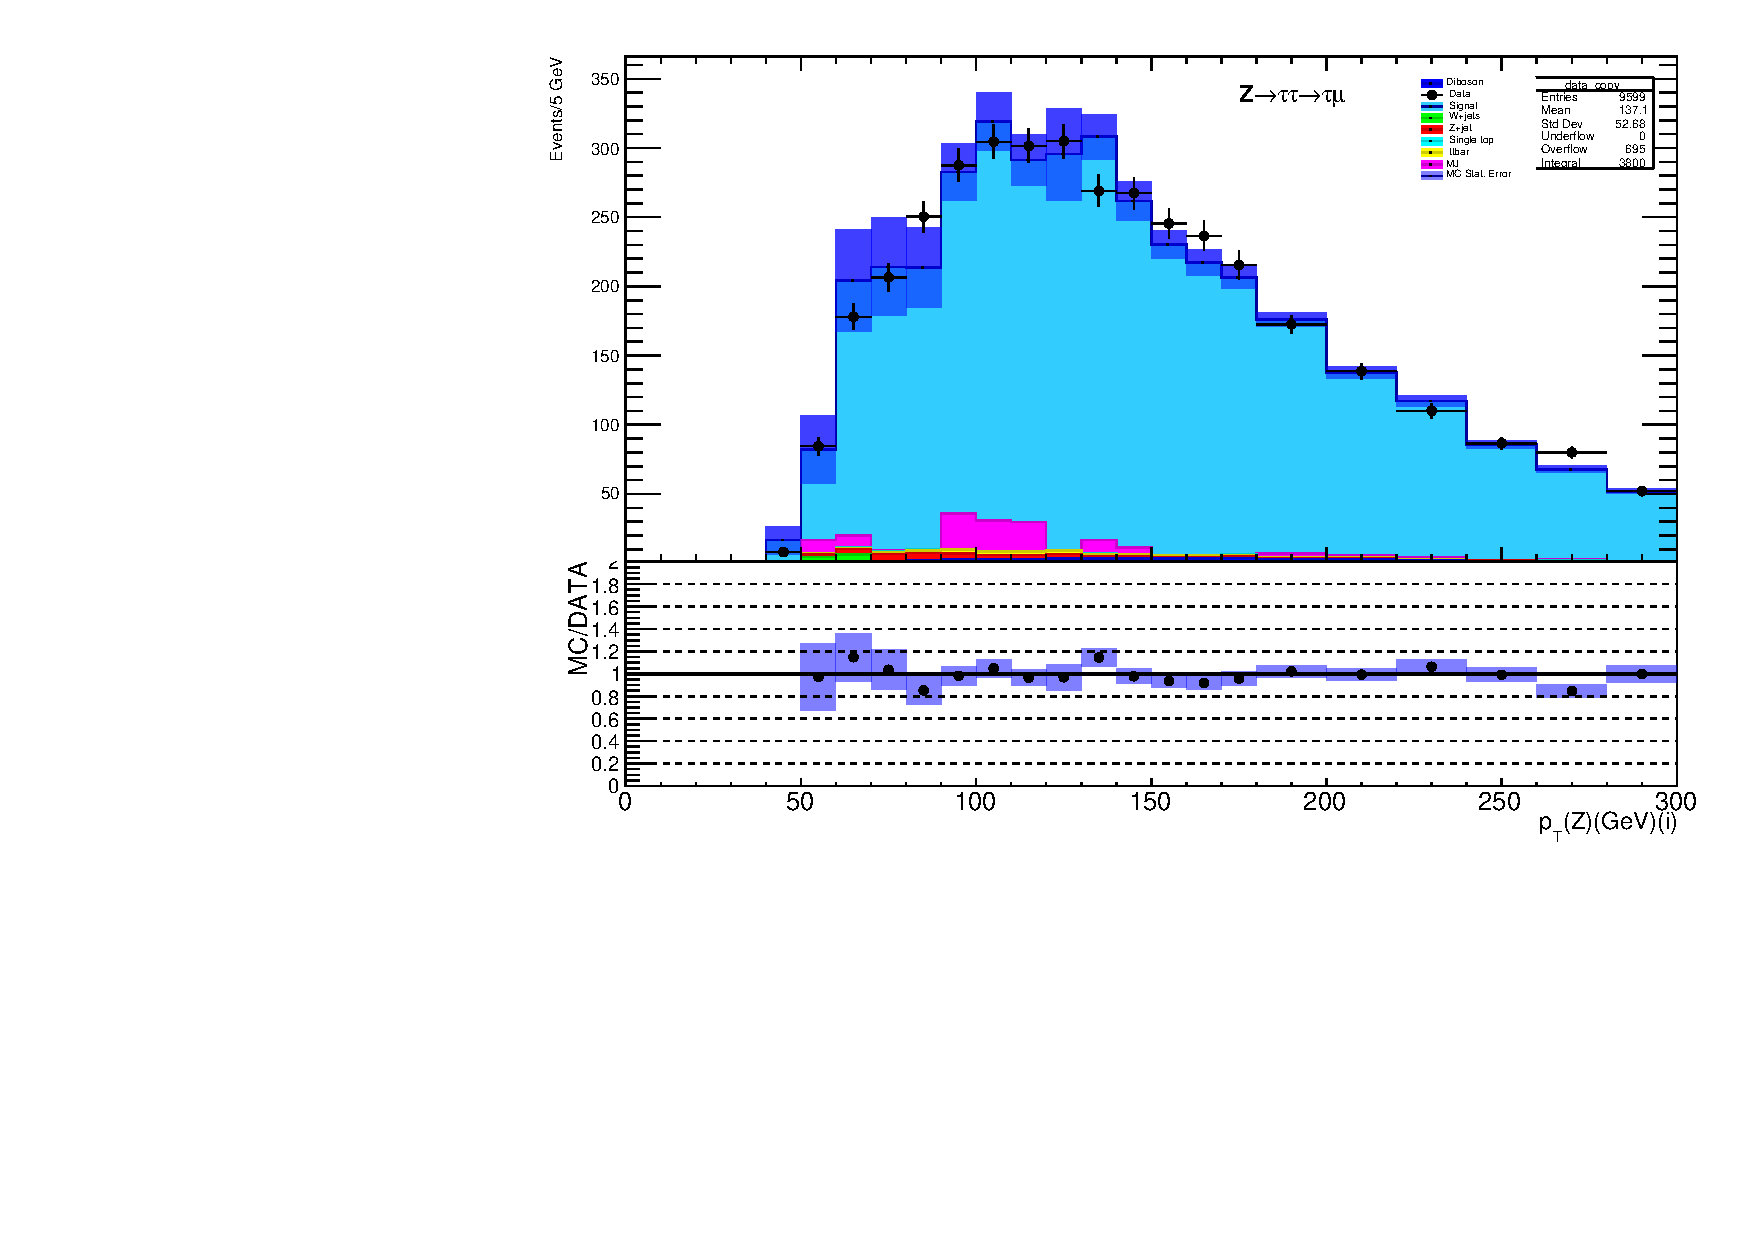
\includegraphics[width=0.50\textwidth]{figures/Fig19a}}}\hfill
	\subfloat[]{\label{Fig21b}{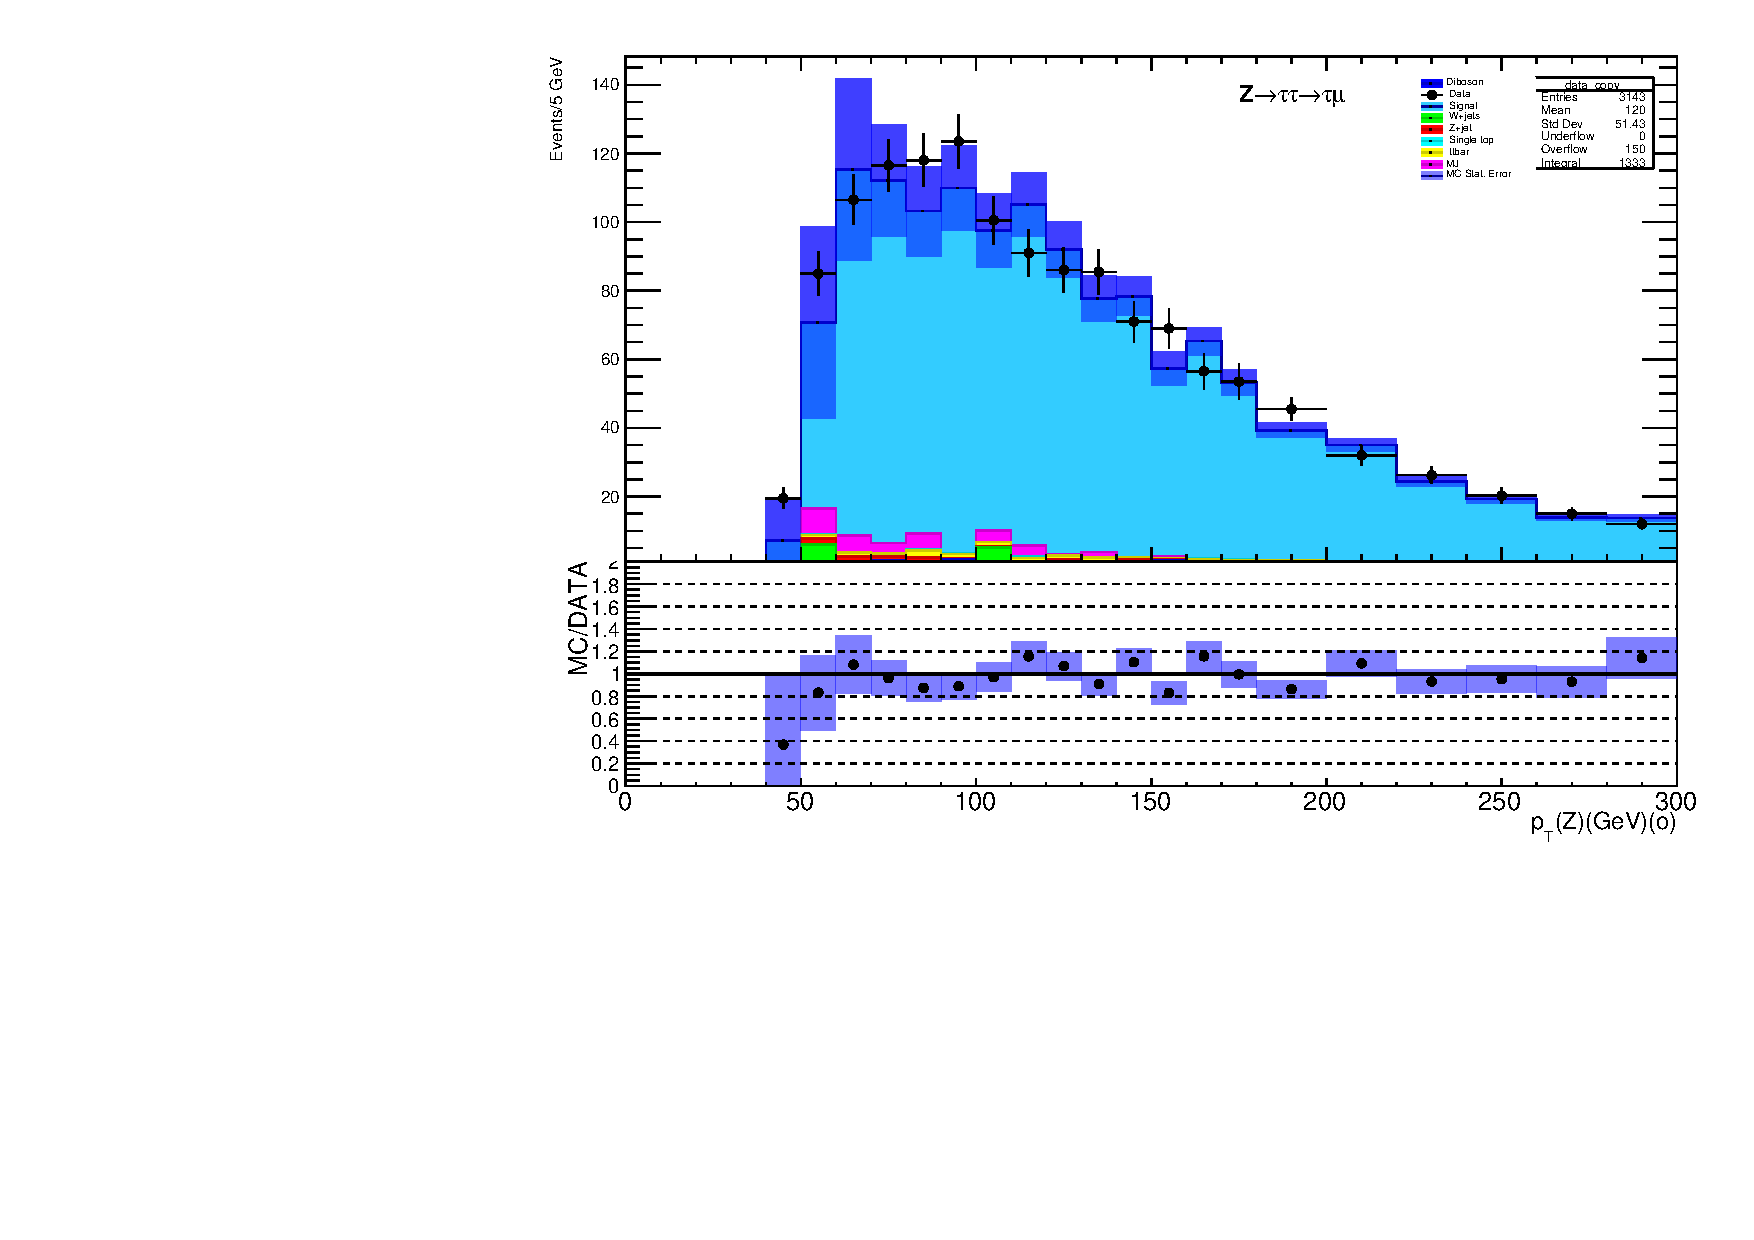
\includegraphics[width=0.50\textwidth]{figures/Fig21}}}\hfill
	\subfloat[]{\label{Fig21c}{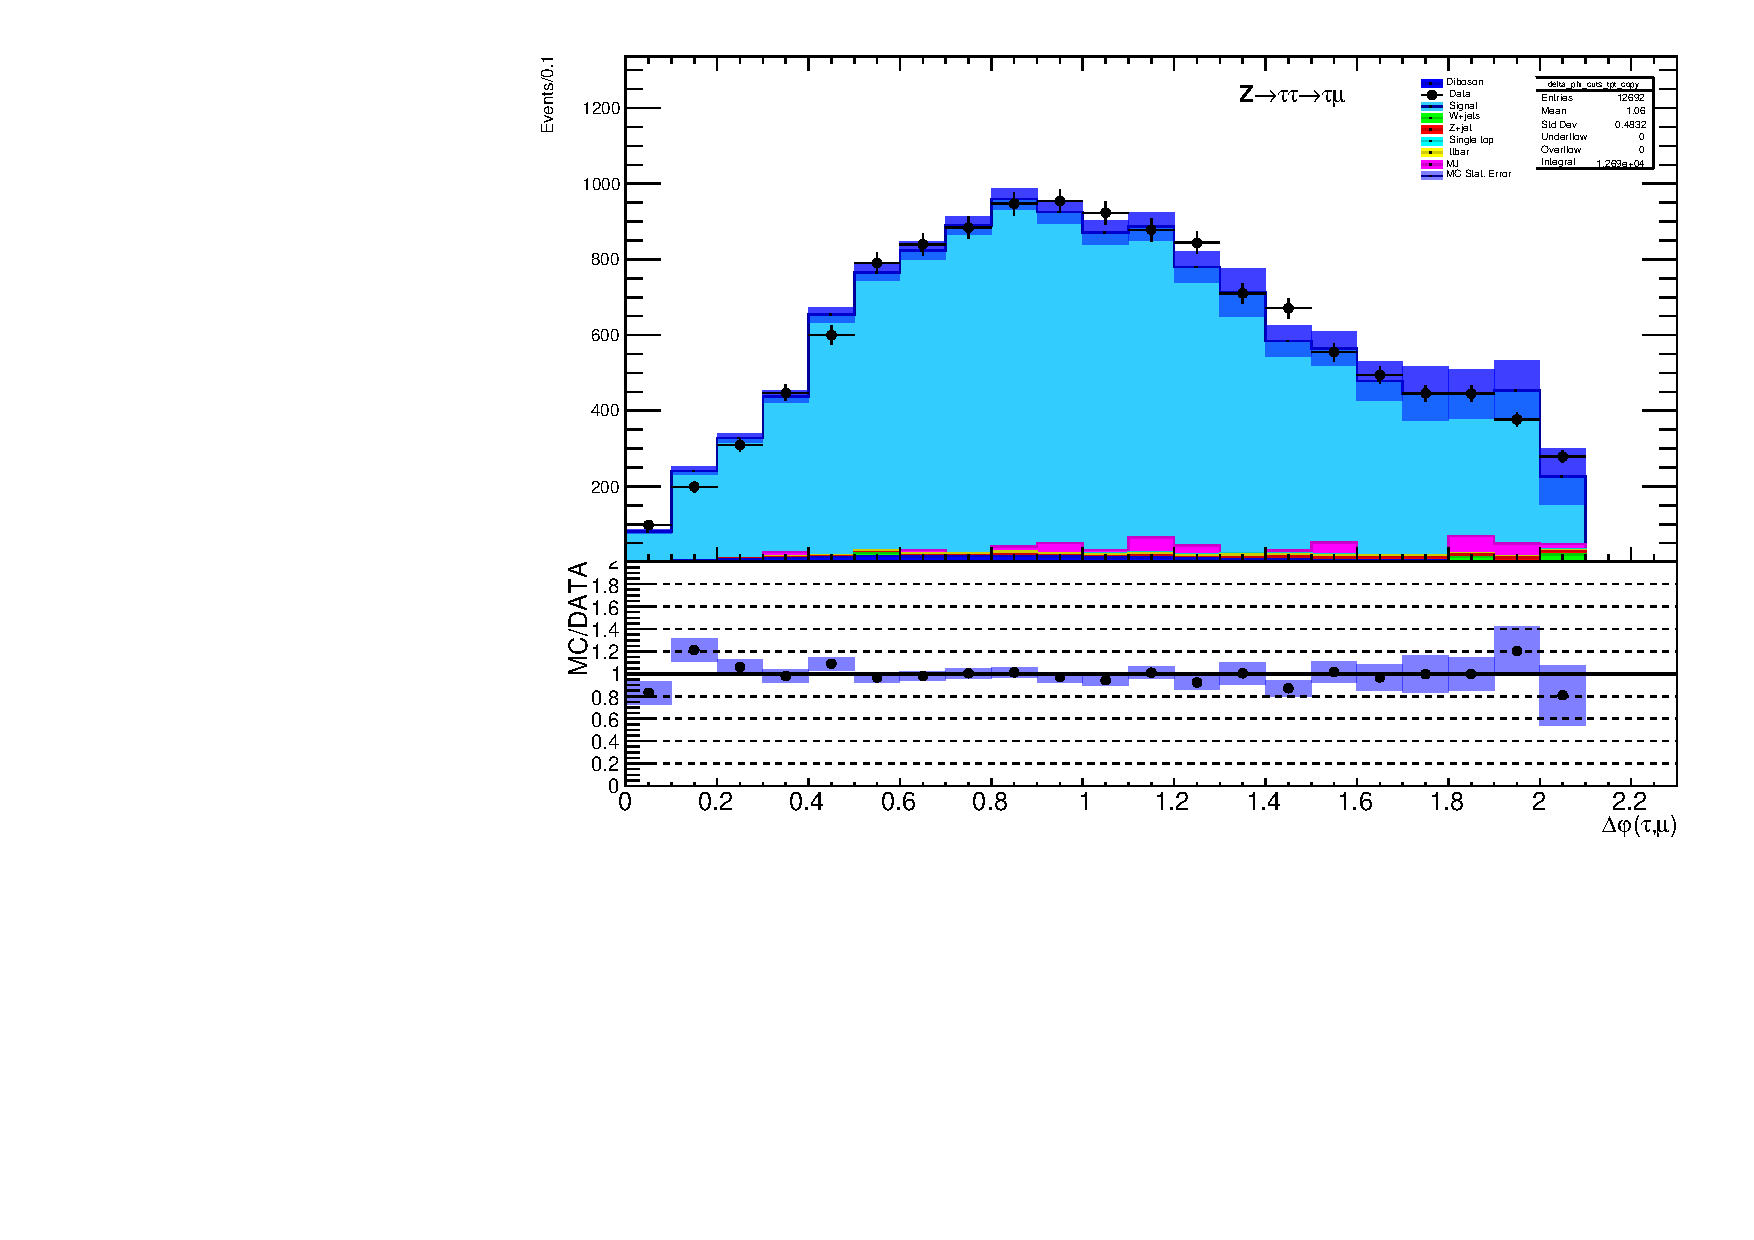
\includegraphics[width=0.50\textwidth]{figures/Fig19b}}}
	\caption{Distribution of Z$(\pt)$ for in-between events (a), Z$(\pt)$ for outside events (b) and $\Delta\phi(\tauh,\mu)$ (c). All the other cuts have been applied apart from the one being plotted.}
	\label{Fig21}
\end{figure}
\begin{figure}[H]
	\centering
	\subfloat[]{\label{Fig22a}{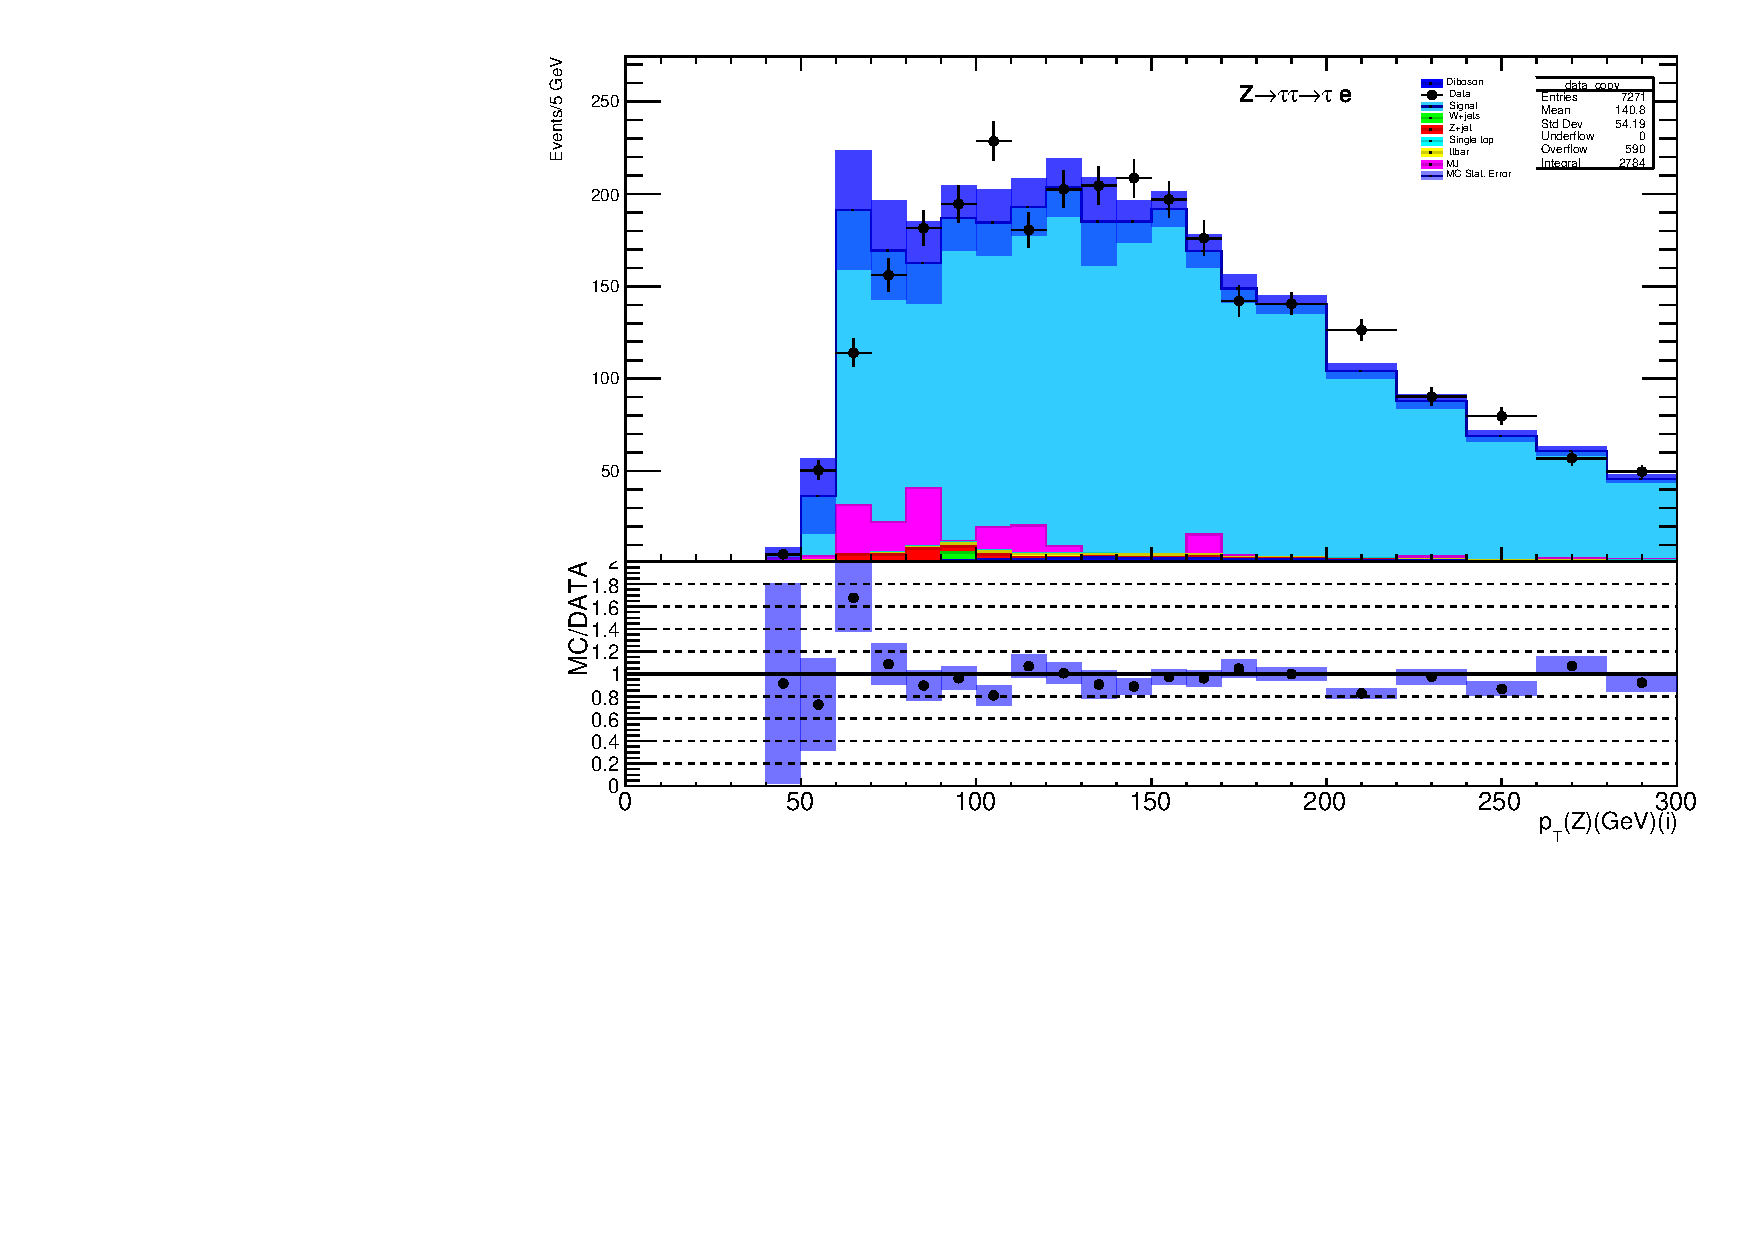
\includegraphics[width=0.50\textwidth]{figures/Fig22a}}}\hfill
	\subfloat[]{\label{Fig22b}{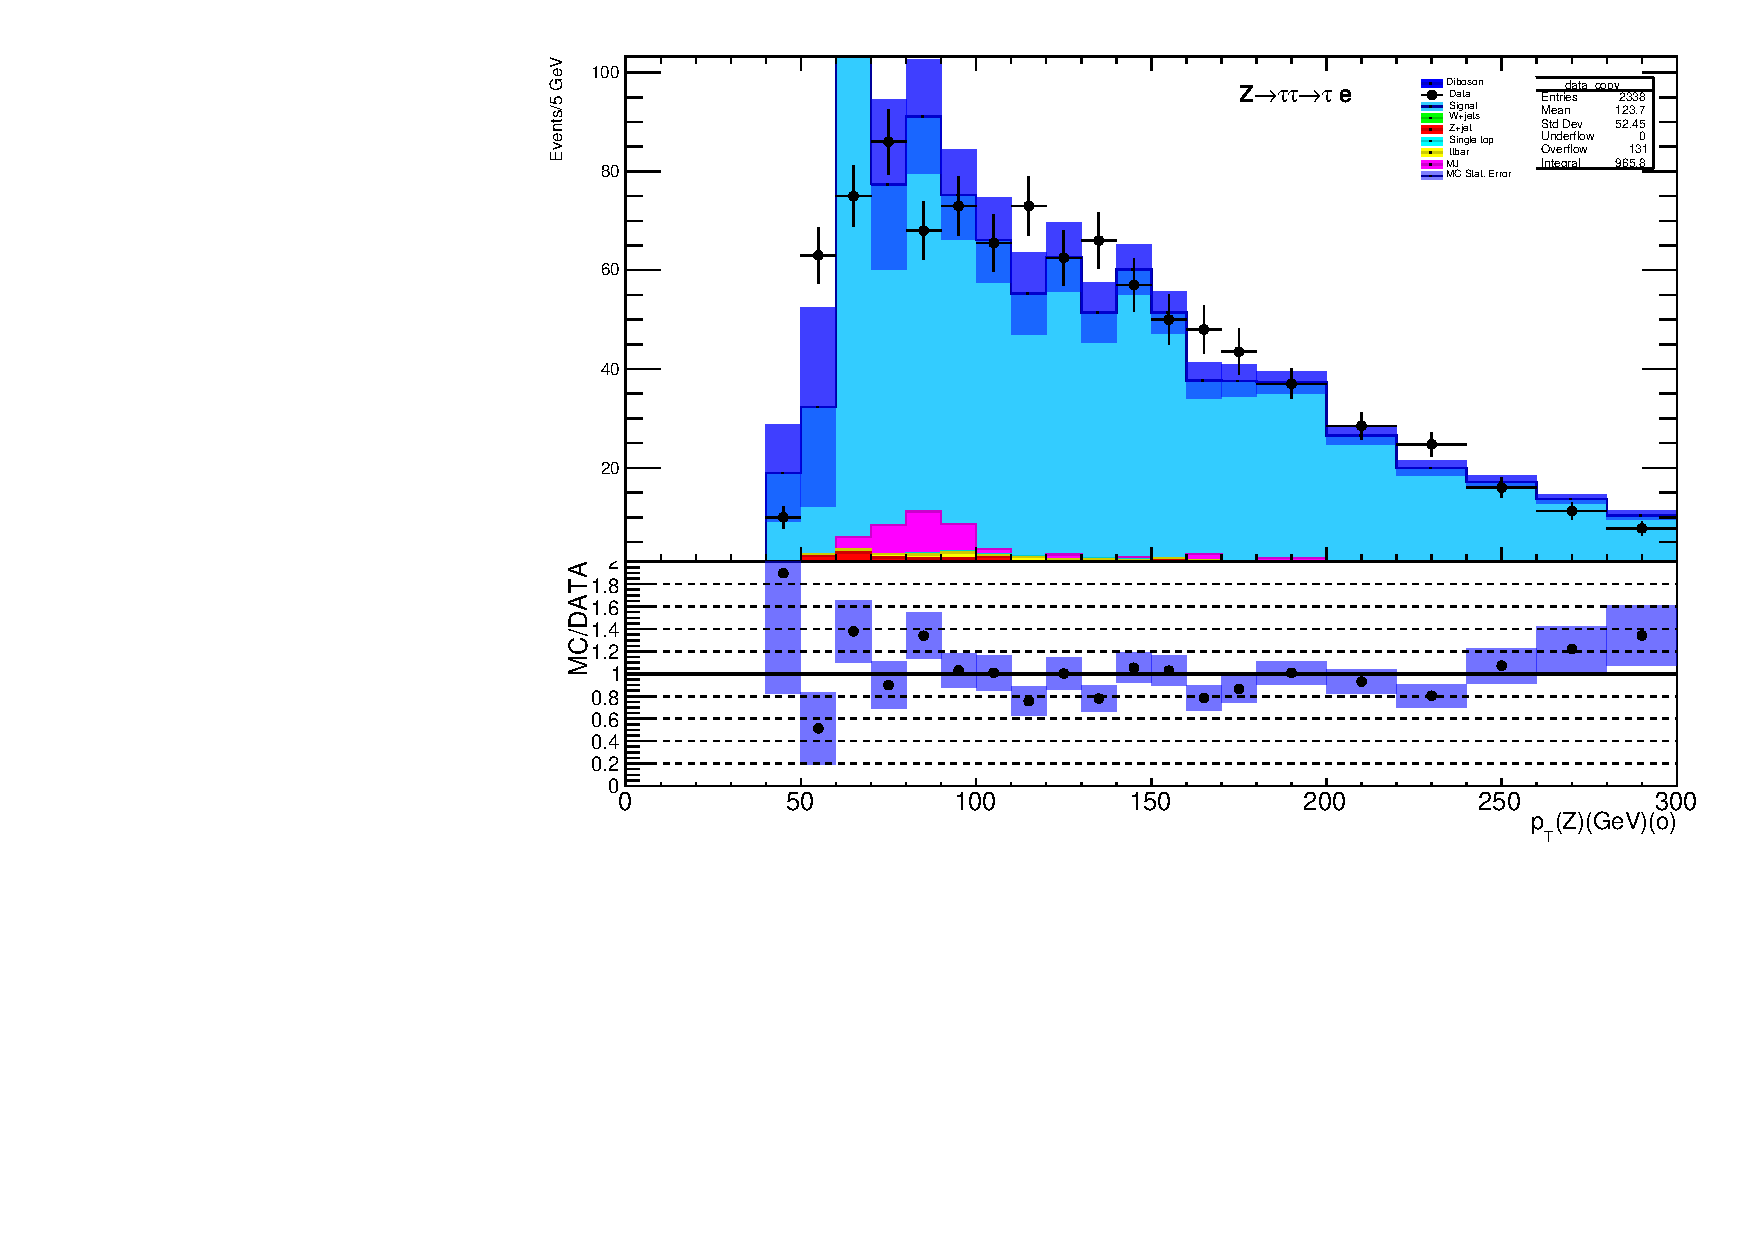
\includegraphics[width=0.50\textwidth]{figures/Fig22b}}}\hfill
	\subfloat[]{\label{Fig22c}{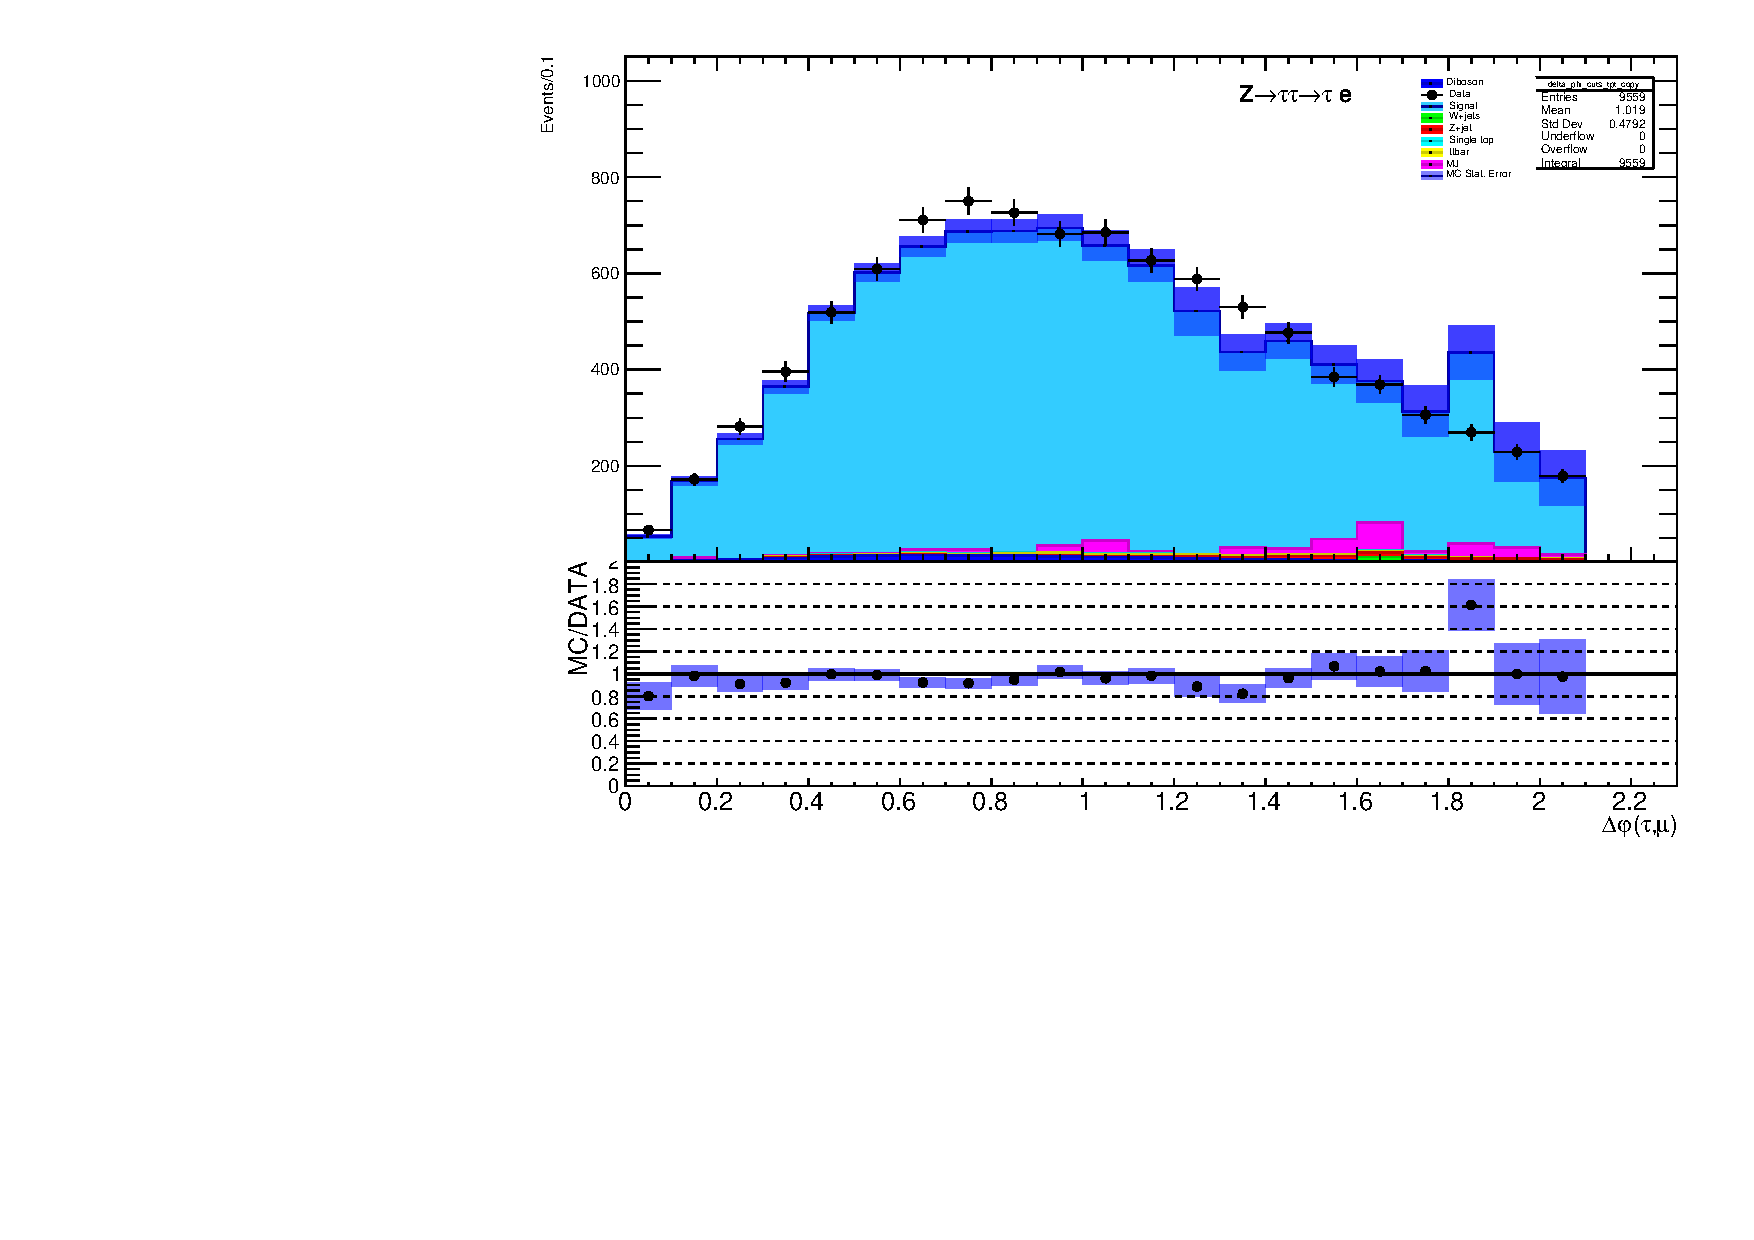
\includegraphics[width=0.50\textwidth]{figures/Fig22c}}}
	\caption{Distribution of Z$(\pt)$ for in-between events (a), Z$(\pt)$ for outside events (b) and $\Delta\phi(\tauh,e)$ (c). All the other cuts have been applied apart from the one being plotted.}
	\label{Fig22}
\end{figure}